\chapter{Stability (35 pages)}
\label{Stability}


\section{Drift}

\section{Dynamics}

\begin{figure}
\begin{center}
 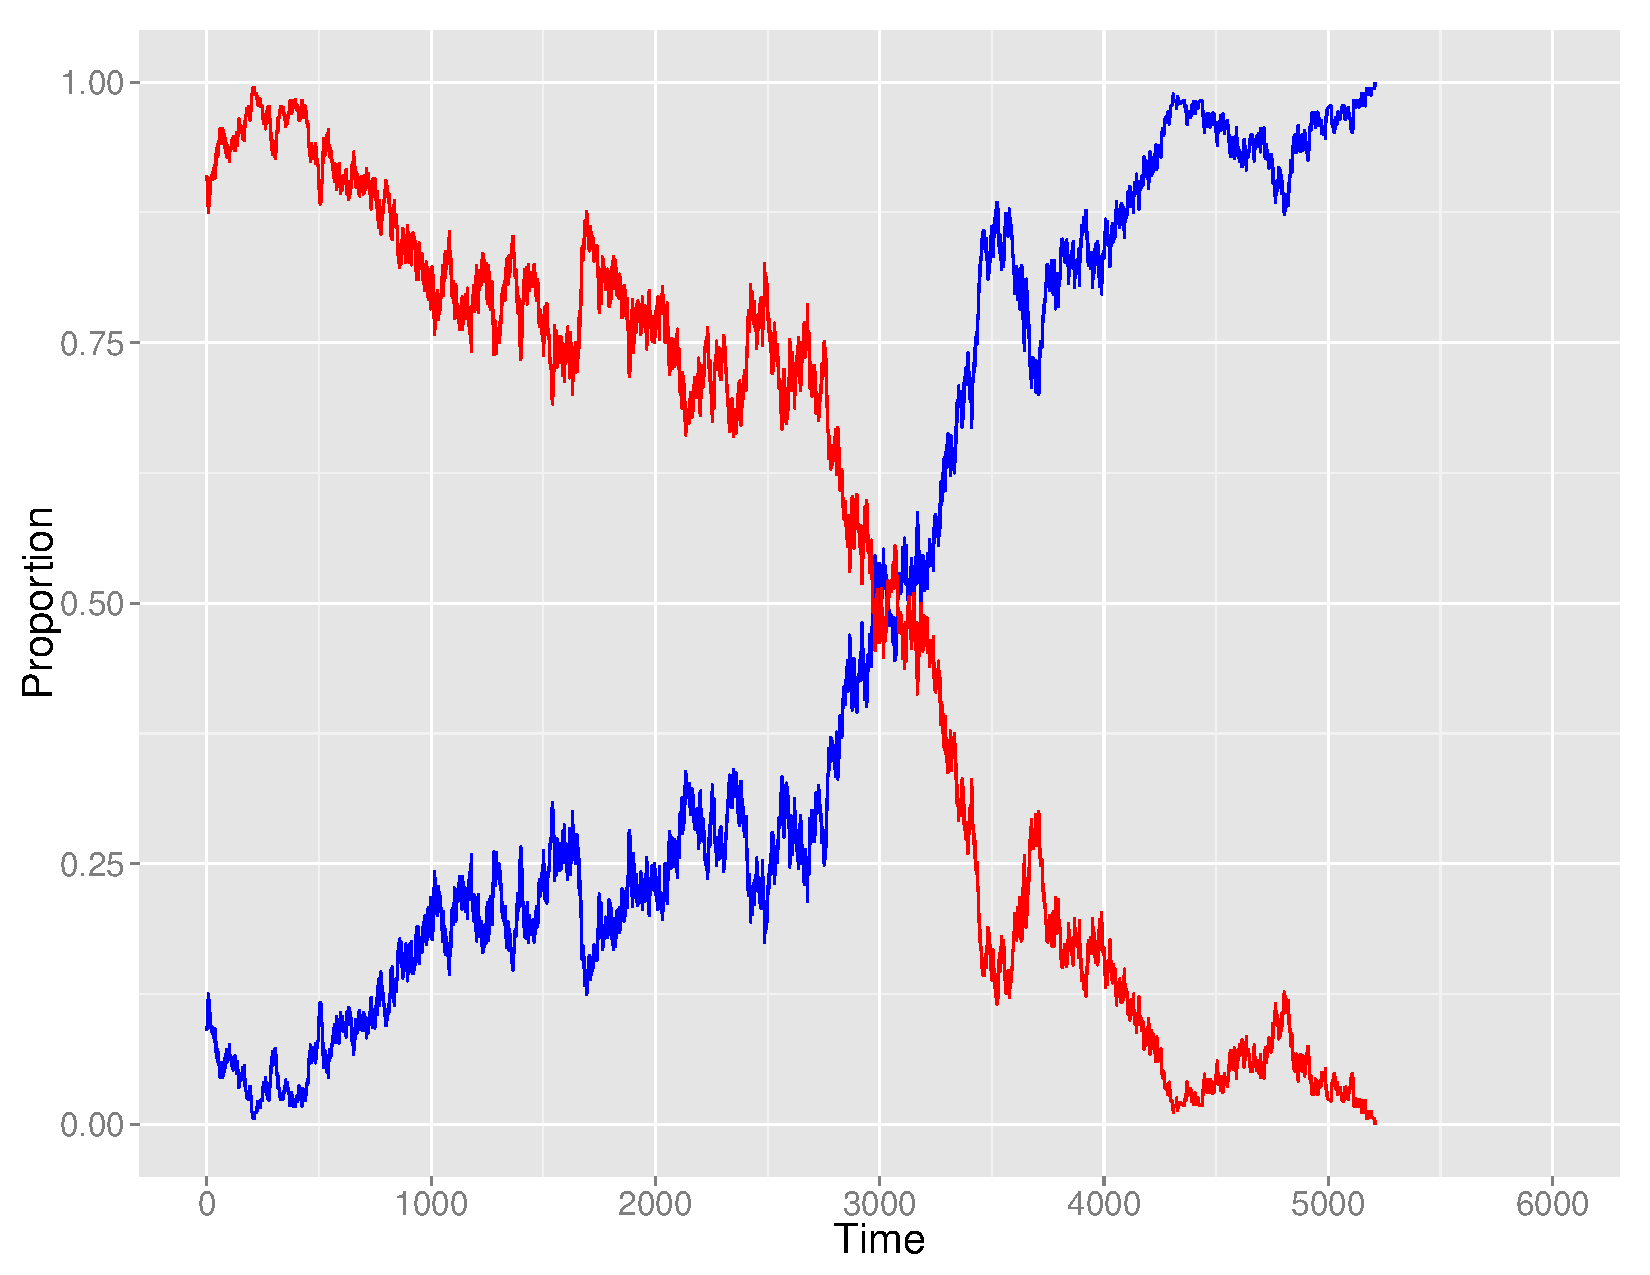
\includegraphics[width=\textwidth]{drift}
\end{center}
	\caption{}
	\label{}
\end{figure}


\begin{figure}
\begin{center}
	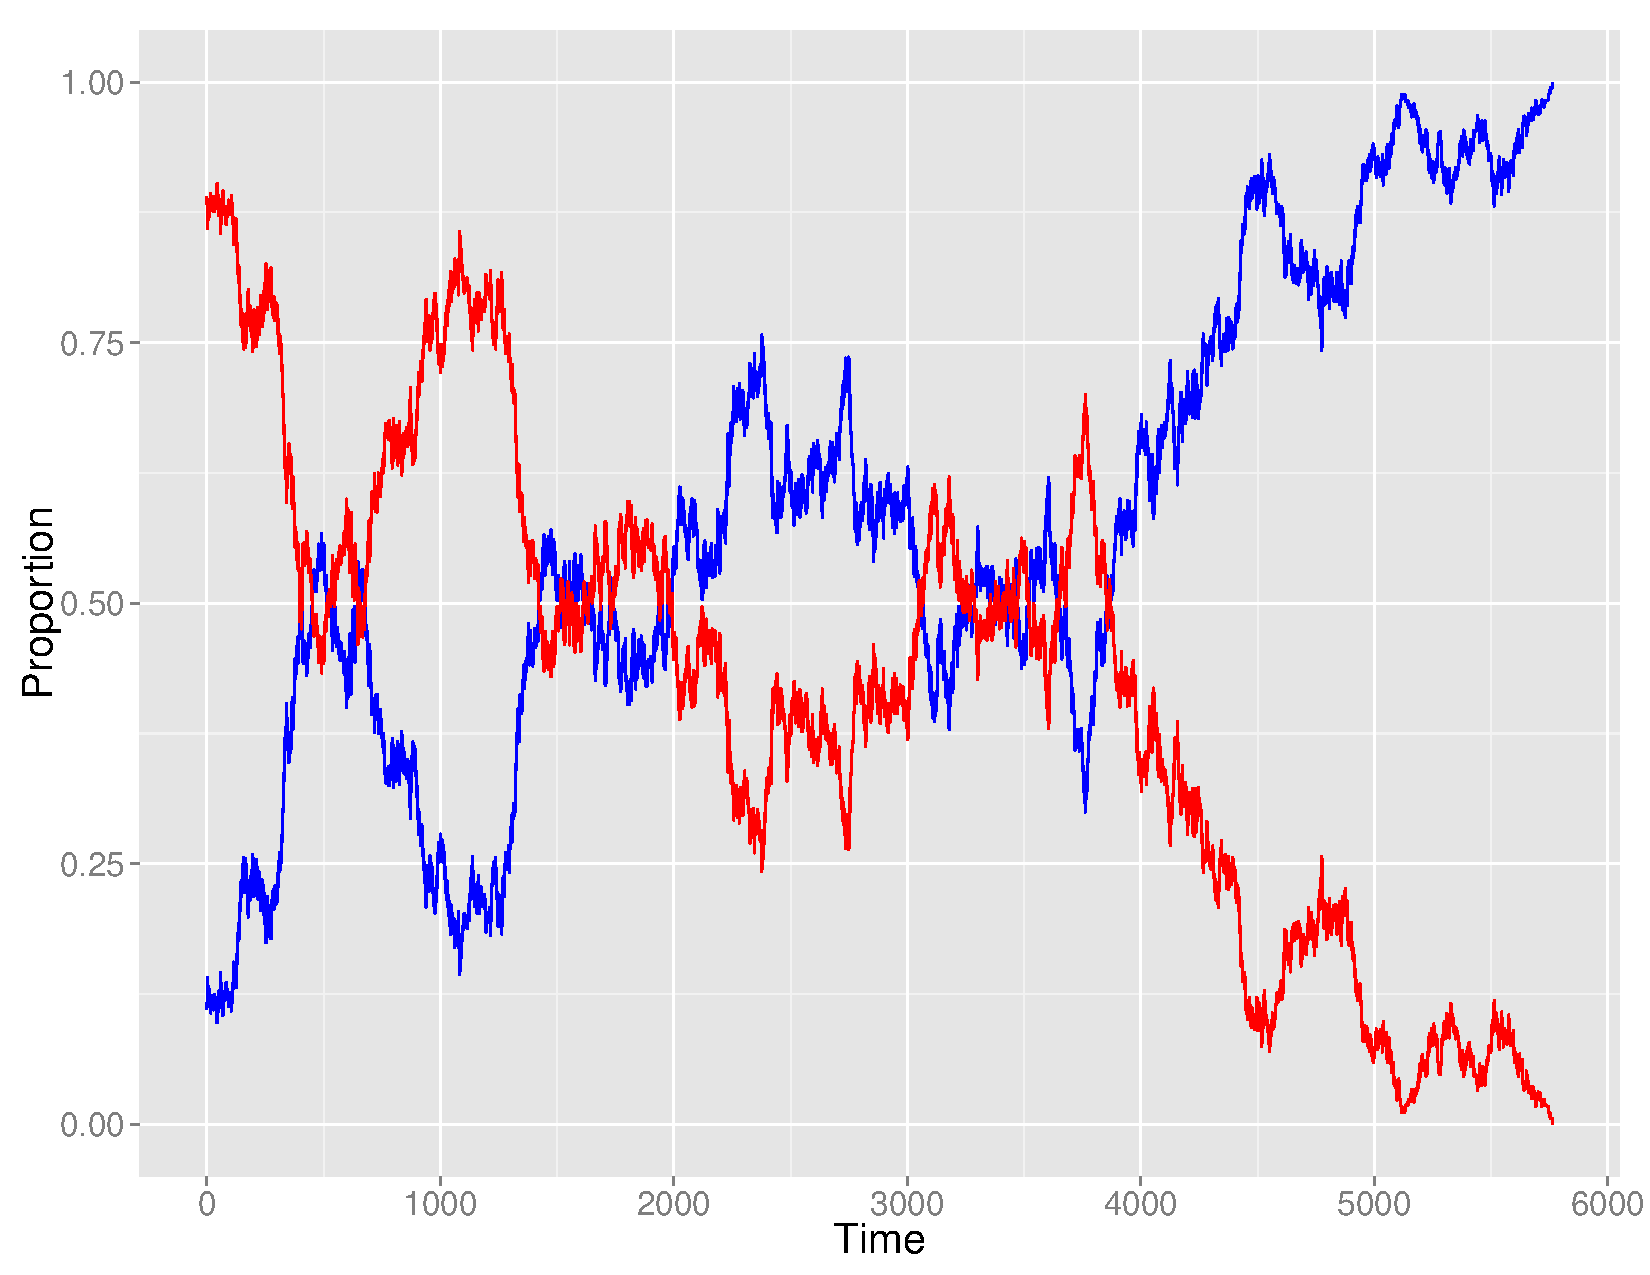
\includegraphics[width=\textwidth]{selection}
\end{center}
	\caption{}
	\label{}
\end{figure}


\section{Data}

Starting in Early Middle English, we find the transition from preverbal to embracing negation taking place. We can trace the proportion of different forms over time as in Figure \ref{neg-three-plot}. Each circle represents tokens in a year. The size of the circle represents the number of tokens negative declaratives. The height of the circle represents the proportion of those instances that are a particular form. Locally-weighted regression lines are fit to these proportions. We see the transition from \textit{\color{red} ne} to \textit{\color{blue} ne...not} starting from around the 12th century. Following close behind, we see the transition from \textit{\color{blue} ne...not} to \textit{\color{green} not} in the 14th century.

\begin{figure}
\centering
     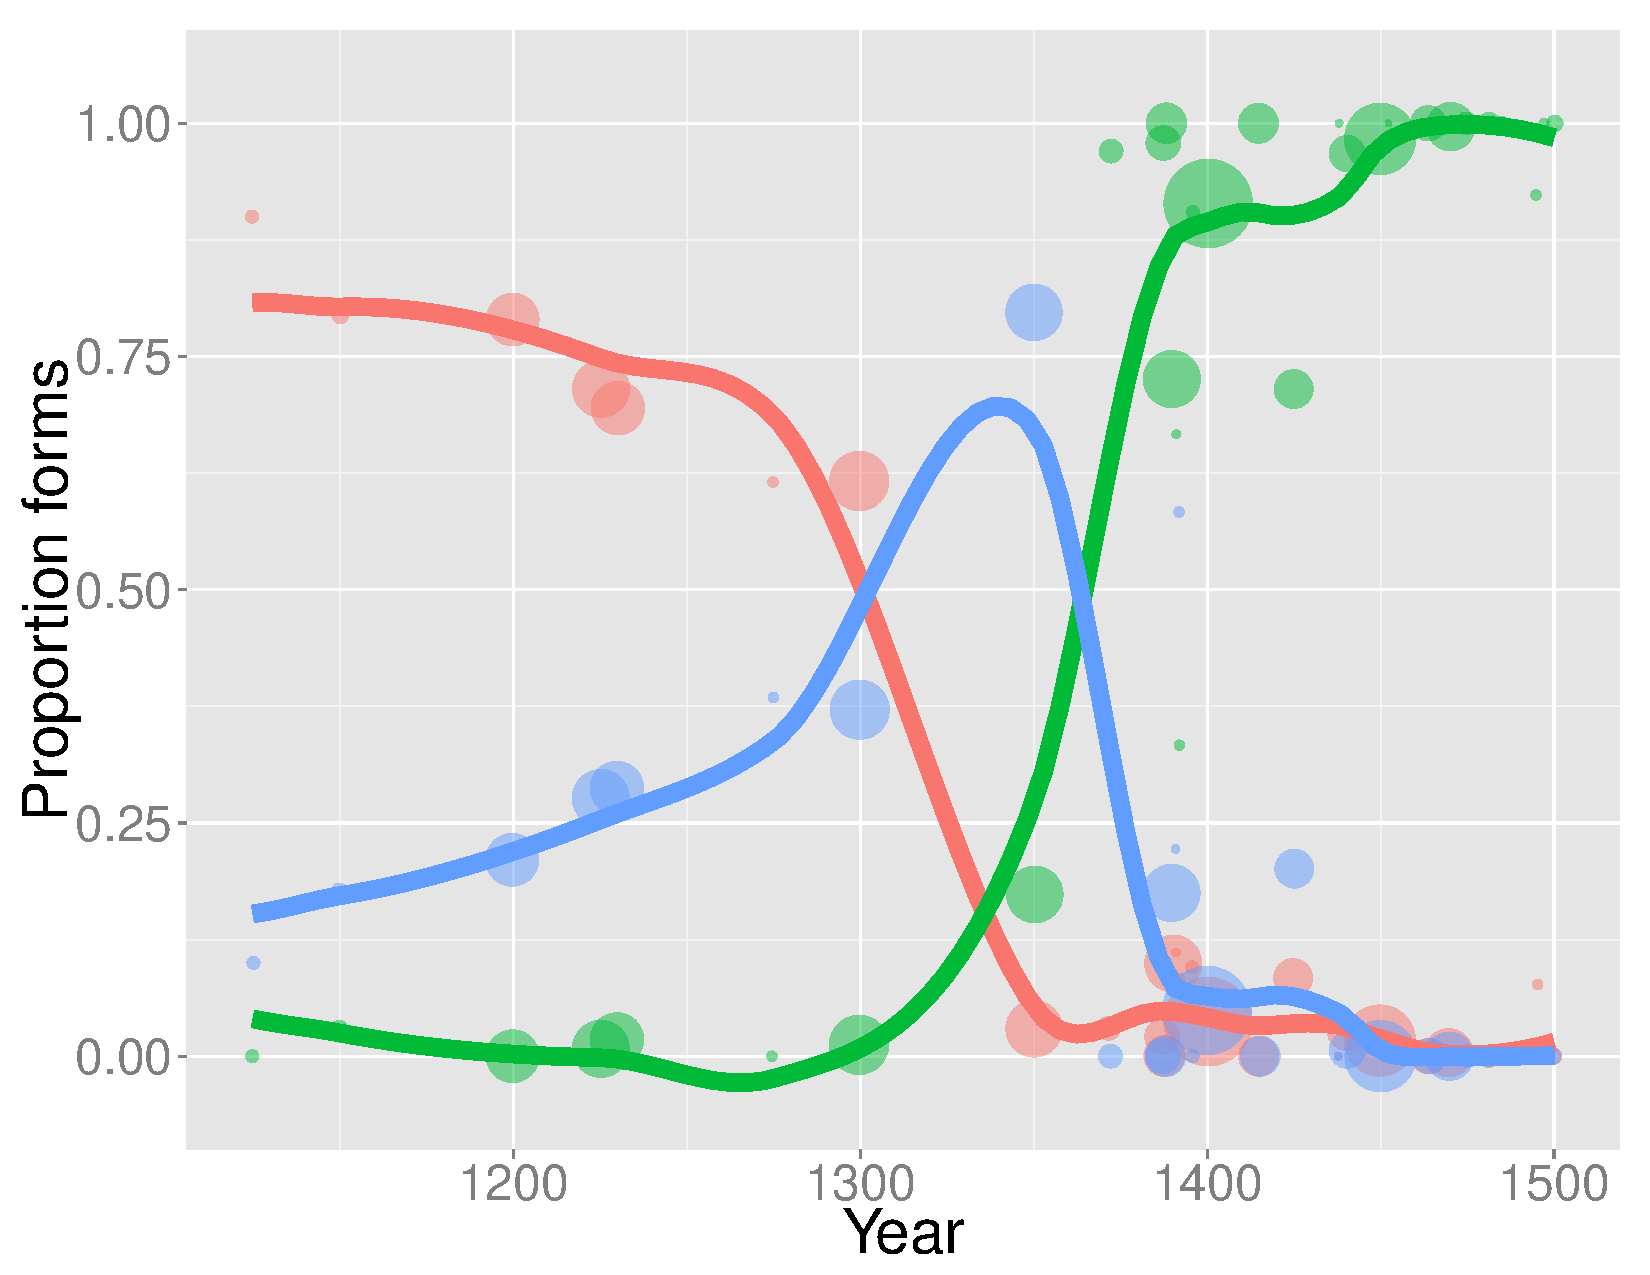
\includegraphics[width=\textwidth]{neg-year-lines.pdf}
\caption{Proportion of forms of negation in Negative Declaratives}
\label{neg-three-plot}
\end{figure}

There are at least two decisions to be made when dealing with the data, which correspond roughly with the ways we'll go about analyzing the data.

First, we have to decide what data should be compared. For example, if we are trying to determine if the first transition is due to selection, should we compare \textit{\color{red} ne} to \textit{\color{blue} ne...not} or should we compare \textit{\color{red} ne} to \textit{\color{blue} ne...not} and \textit{\color{green} not} grouped together? If we do the former, it's pretty clear that the variation beyond 1350 has less to do with the selection of \textit{\color{red} ne} versus \textit{\color{blue} ne...not}, but rather with\textit{\color{green} not} becoming the majority variant. Taking the latter route, and lumping \textit{\color{blue} ne...not} and \textit{\color{green} not} together for the sake of comparison solves this problem.

Second, we have to decide the period of time in which the comparison is being made. This offers another solution to the problem posed above. Namely, if we only compare \textit{\color{red} ne} to \textit{\color{blue} ne...not} prior to 1350 or so we don't have to worry about any noisy  data after that point. There are some natural reasons for choosing a cut-off point. For example, if we are only comparing \textit{\color{red} ne} and \textit{\color{blue} ne...not}, it would seem reasonable to only compare them  when together they constitute the majority of the tokens for a given year. For both transitions, we have the same exact point at 1350, which means we'll be using these tokens for both sets of tests.

We'll try both ways of analyzing the data. First, we'll lump the forms together comparing the pre-verbal to the embracing and post-verbal form, and the pre-verbal and embracing forms to the post-verbal form. We'll do this with all of the data. Second, we'll split the variants, only comparing two forms at a time, before and after 1350.

\subsection{Lumping}

The proportion of \textit{\color{blue} ne...not} and \textit{\color{green} not} forms combined over time can be seen in Figure \ref{lump-plot1}. The results of running the FIT on variable-width bins is shown in Table \ref{lump-table1}. For any binning finer than nine, we find either that an absorption event occurs or there are non-unique ways of binning the data by quantiles.


\begin{figure}
\centering
     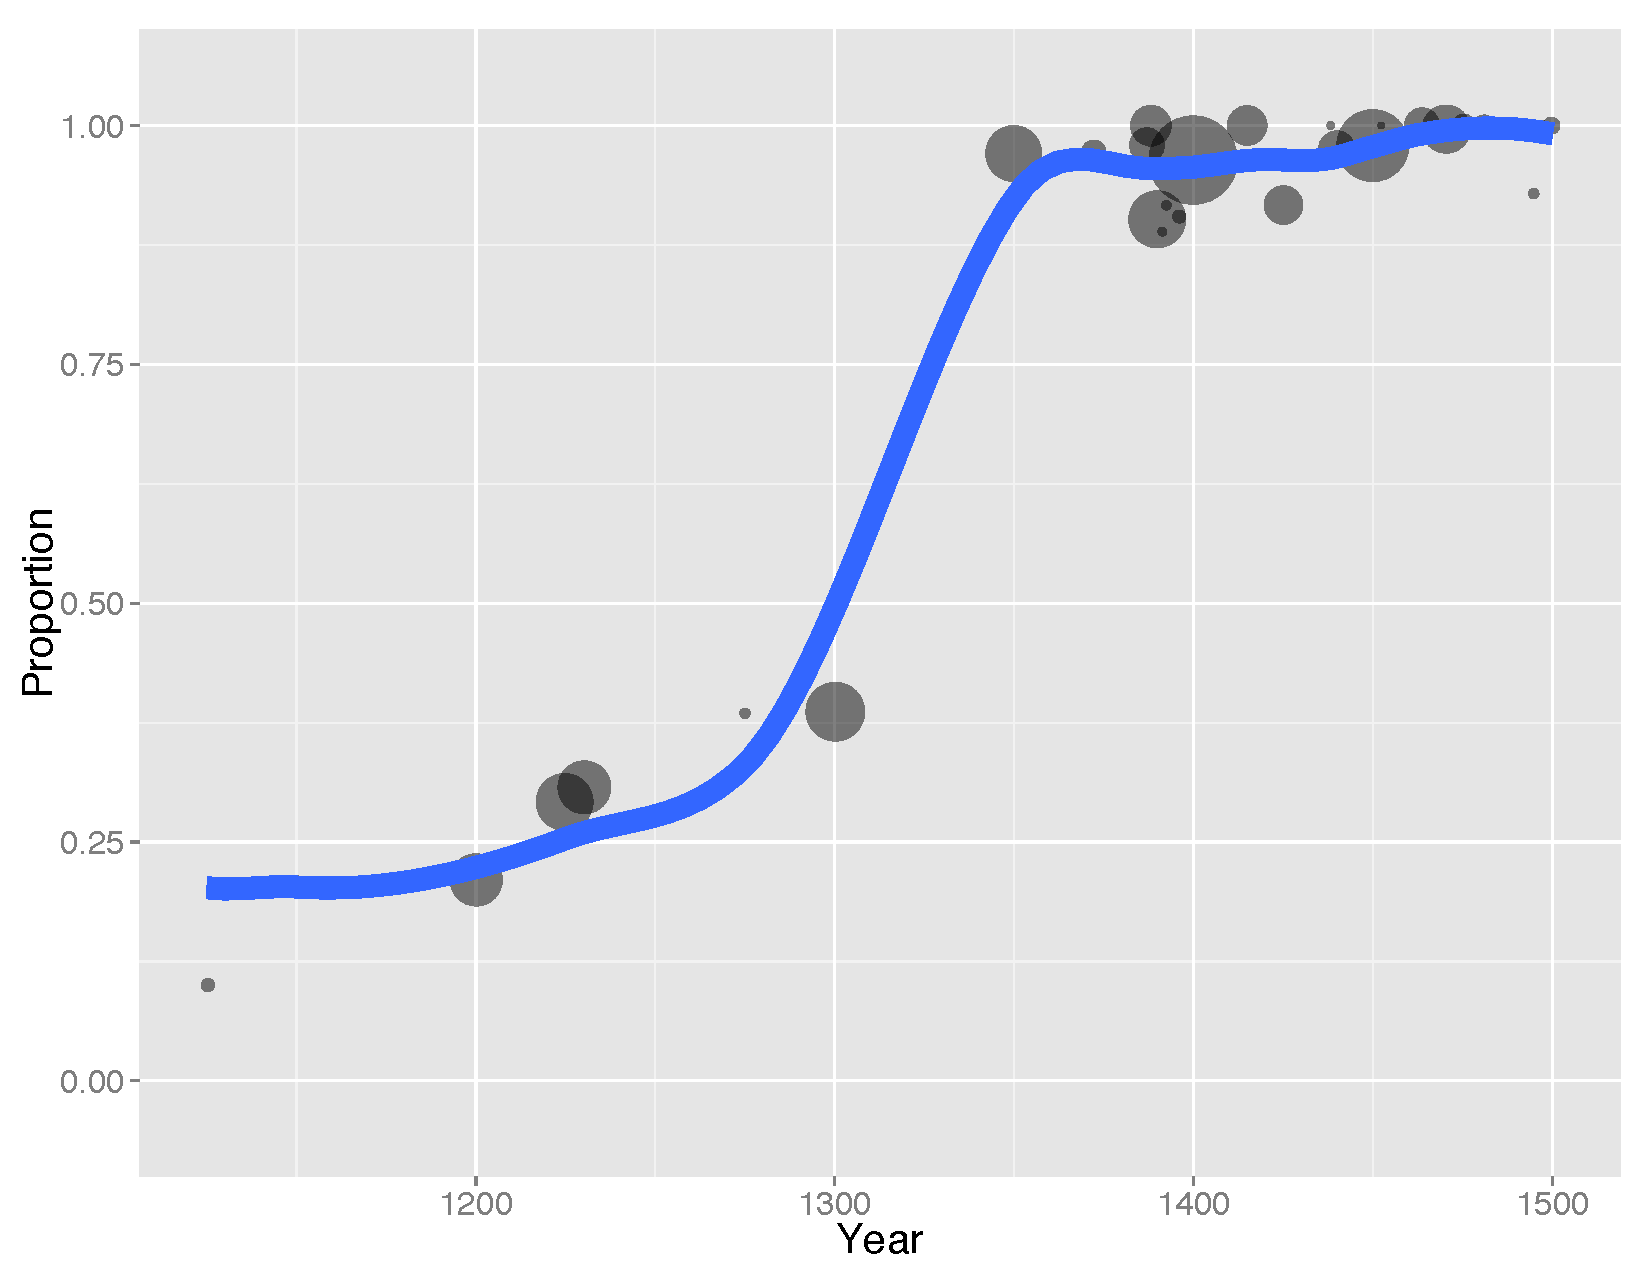
\includegraphics[width=\textwidth]{lump-plot1.pdf}
\caption{Proportion of \textit{\color{blue} ne...not} and \textit{\color{green} not}  versus  \textit{\color{red}  ne} over time}
\label{lump-plot1}
\end{figure}


\begin{table}[ht]
\centering
\begin{tabular}{c  l  r  l  l  l  l   r  r  l l }
  \hline
Bins & ML$s$ & ML$\alpha$ & LRT-P & $\overline{Y}$ & $t_{FI}$ & FIT-P & $\mu$ & $\sigma_n$ & SW-P & WX-P \\ 
  \hline
  4 & 0.02507 & 3270 & 0.000075 & 0.0345 & 1.3269 & 0.1579 & 1368 & 157 & 0.1691 & 0.1250 \\  
  5 & -- & -- & -- & 0.0331 & 2.5445 & 0.0422 & 1094 & 278 & 0.1406 & 0.0625 \\  
  6 & 0.01913 & 15900 & 0.000023 & 0.0278 & 2.6394 & 0.0288 & 912 & 197 & 0.2050 & 0.0312 \\ 
  7 & -- & -- & -- & 0.0238 & 2.4347 & 0.0295 & 781 & 236 & 0.2185 & 0.0313 \\
  8 & -- & -- & -- & 0.0223 & 1.4884 & 0.0936 & 684 & 129 & 0.1619 & 0.0781 \\ 
   \hline
\end{tabular}
\caption{FIT on \textit{\color{red}  ne} versus \textit{\color{blue} ne...not} and \textit{\color{green} not} }
\label{lump-table1}
\end{table}


The proportion of \textit{\color{green} not} forms over time can be seen in Figure \ref{lump-plot2}. The results of running the FIT on variable-width bins is shown in Table \ref{lump-table2}. Again, for any binning finer than nine, we find either that an absorption event occurs or there are non-unique ways of binning the data by quantiles.


\begin{figure}
\centering
     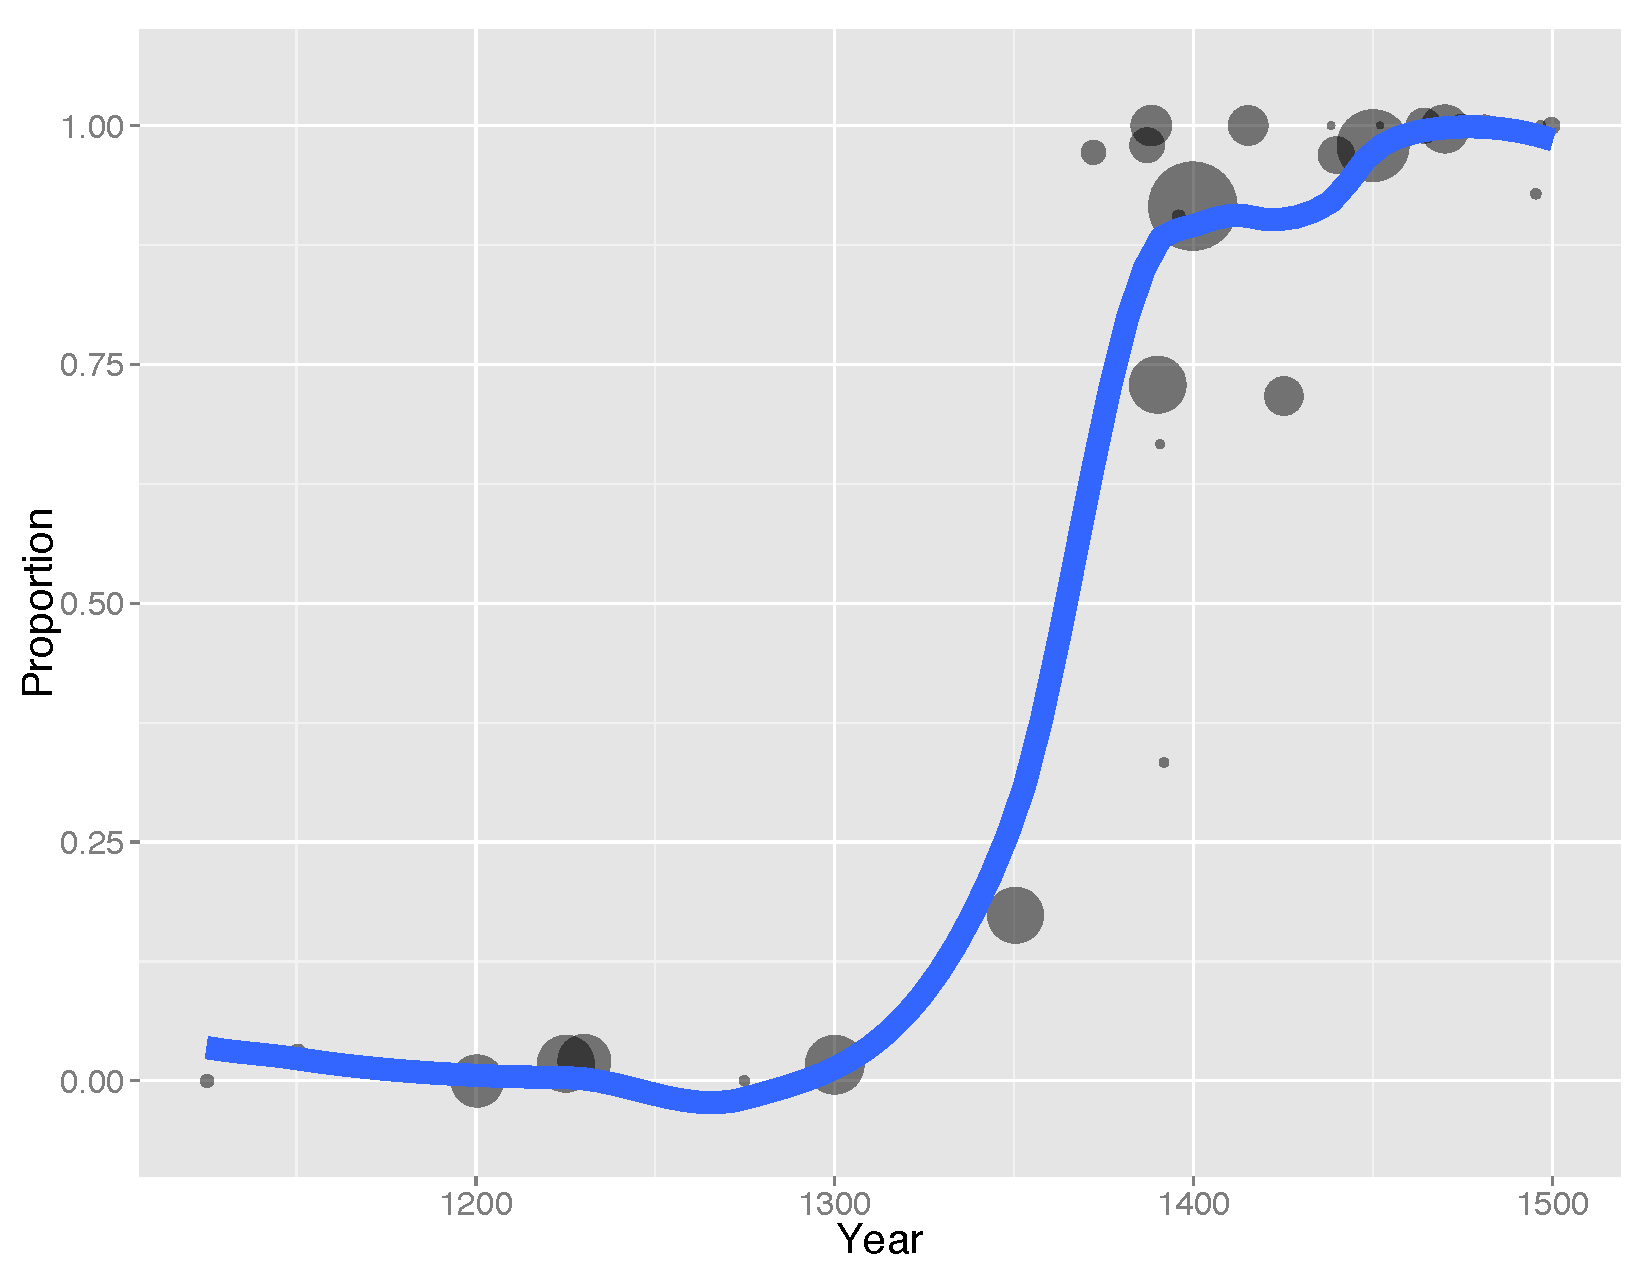
\includegraphics[width=\textwidth]{lump-plot2.pdf}
\caption{Proportion of \textit{\color{green} not} versus \textit{\color{red}  ne} and \textit{\color{blue} ne...not} over time}
\label{lump-plot2}
\end{figure}


\begin{table}[ht]
\centering
\begin{tabular}{c  l  r  l  l  l  l   r  r  l l }
  \hline
Bins & ML$s$ & ML$\alpha$ & LRT-P & $\overline{Y}$ & $t_{FI}$ & FIT-P & $\mu$ & $\sigma_n$ & SW-P & WX-P \\
  \hline
  4 & 0.05791 & 15660 & 0.000045 & 0.1316 & 1.3857 & 0.1501 & 1368 & 157 & 0.1135 & 0.1250 \\
  5 & 0.11907 & 24 & 0.000068 & 0.0825 & 1.9787 & 0.0711 & 1094 & 278 & 0.1300 & 0.0625 \\ 
  6 & -- & -- & --  & 0.0624 & 1.7021 & 0.0820 & 912 & 197 & 0.0052 & 0.0312 \\
  7 & -- & -- & -- & 0.0520 & 1.5250 & 0.0939 & 781 & 236 & 0.0421 & 0.0781 \\ 
  8 & -- & -- & --  & 0.0649 & 1.8516 & 0.0568 & 684 & 129 & 0.0157 & 0.0781 \\    \hline
\end{tabular}
\caption{FIT on \textit{\color{red}  ne} and \textit{\color{blue} ne...not} versus  \textit{\color{green} not} }
\label{lump-table2}
\end{table}


Together, these results suggest the following. First, in some cases we can reject the null hypothesis of drift in favor of selection for the first transition (Table \ref{lump-table1}). Second, we never find sufficient evidence to reject the null hypothesis for the second transition (Table \ref{lump-table2}). Finally, we should note that  the increments for the second transition are not normally distributed as we bin more finely.


%%%%%%%%%%%%%%%%%%%%%%%%%%%%%%%%%%%%%%%%%%
\subsection{Splitting}

If we choose to split the date by date, we limit the number of tokens available and thus how finely we can bin. The proportion of \textit{\color{blue} ne...not}  versus \textit{\color{red} ne} forms over time can be seen in Figure \ref{split-plot1}. The results of running the FIT on variable-width bins is shown in Table \ref{split-table1}. Binning the data into more than six bins is not possible due to either  non-uniquely defined bins, or absorption events. This is not altogether surprising, given that we can only manage eight or so bins with all of the data, as we did above.


\begin{figure}
\centering
     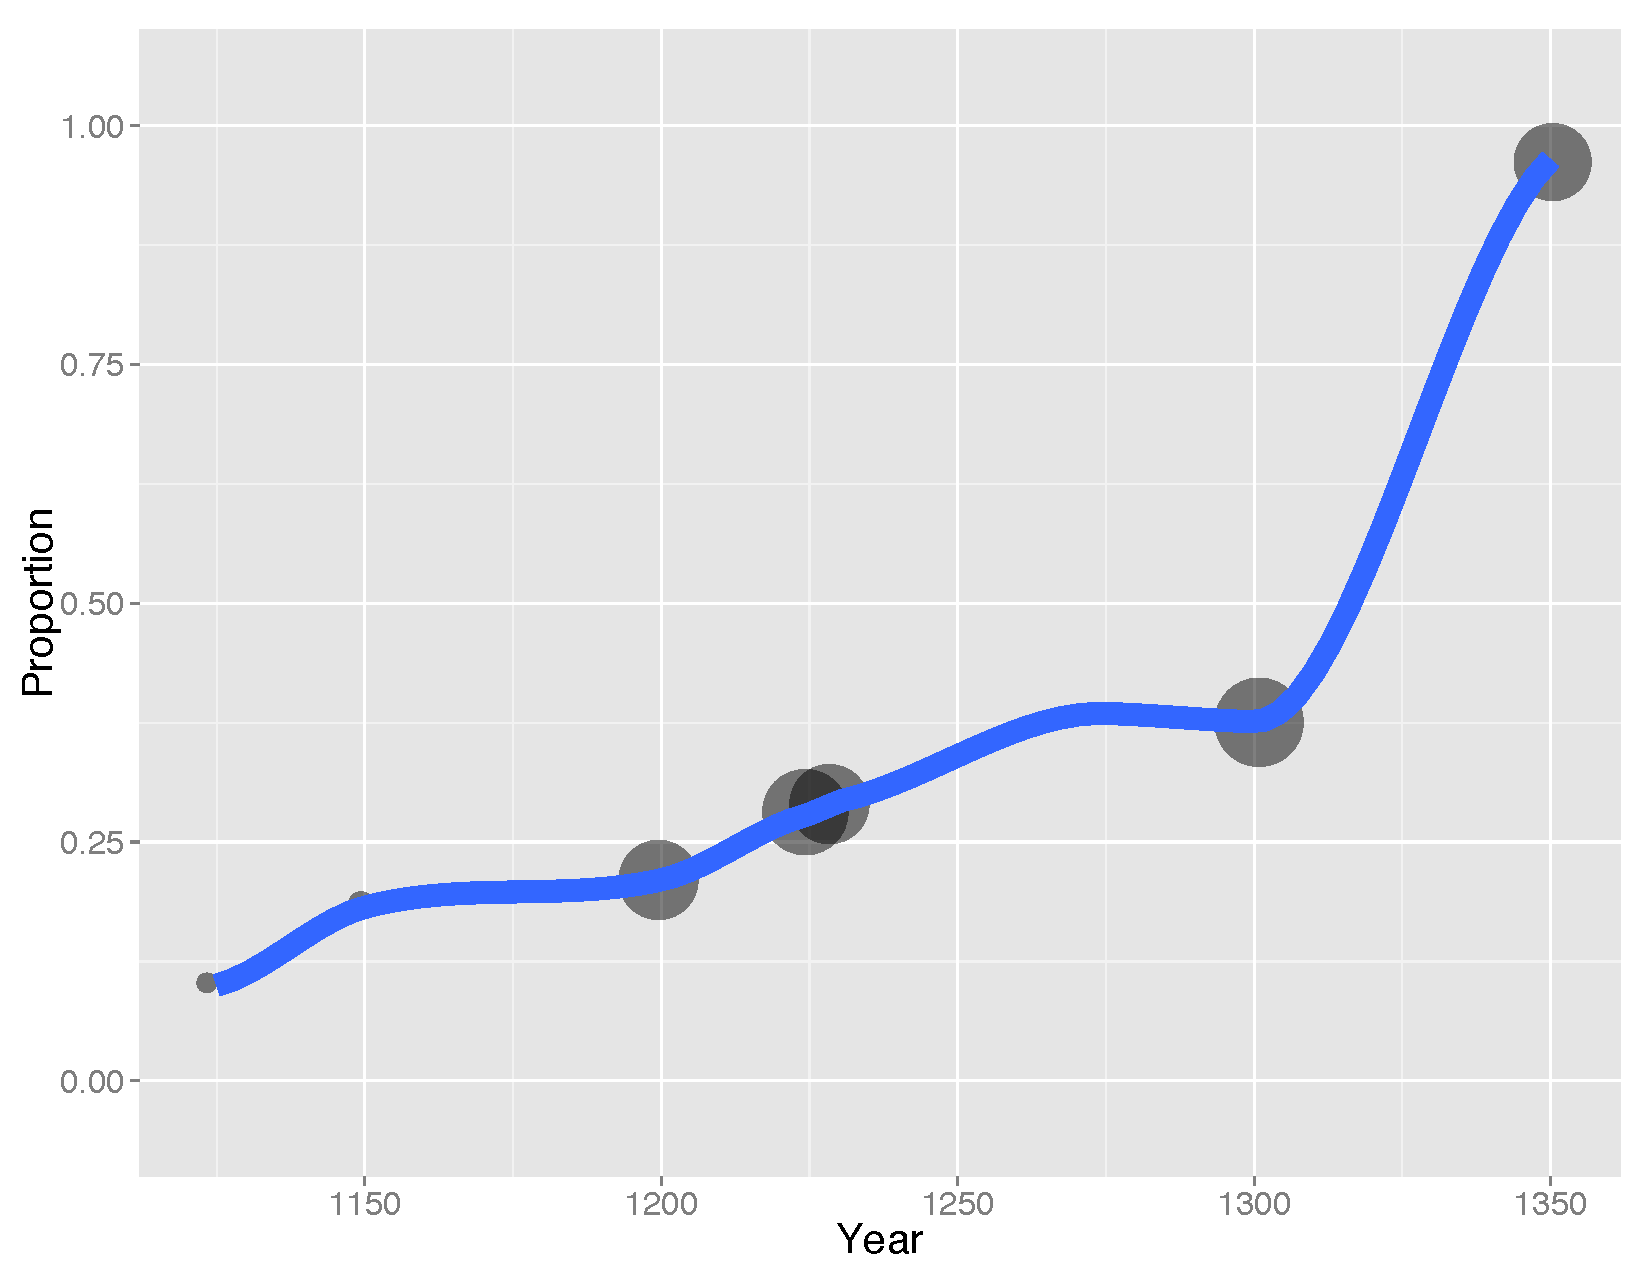
\includegraphics[width=\textwidth]{split-plot1.pdf}
\caption{Proportion of \textit{\color{blue} ne...not}  versus  \textit{\color{red}  ne} until and including 1350}
\label{split-plot1}
\end{figure}

\begin{table}[ht]
\centering
\begin{tabular}{c  l  r  l  l  l  l   r  r  l  l}
  \hline
Bins & ML$s$ & ML$\alpha$ & LRT-P & $\overline{Y}$ & $t_{FI}$ & FIT-P & $\mu$ & $\sigma_n$ & SW-P & WX-P\\ 
  \hline
  4 & 0.02656 & 262 & 0.10 & 0.0480 & 1.5199 & 0.1339 & 454 & 209 & 0.1587 & 0.1250 \\ 
  5 & 0.01140 & 304 & 0.023 & 0.0458 & 1.4588 & 0.1204 & 363 & 38 & 0.0248 & 0.0625 \\
   \hline
\end{tabular}
\caption{FIT on \textit{\color{blue} ne...not}  versus  \textit{\color{red}  ne} until and including 1350}
\label{split-table1}
\end{table}

The proportion of \textit{\color{green} not}  versus \textit{\color{blue} ne...not} forms over time can be seen in Figure \ref{split-plot2}. The results of running the FIT on variable-width bins is shown in Table \ref{split-table2}. Again, binning the data into more than six bins is not possible due to either  non-uniquely defined bins, or absorption events.

\begin{figure}
\centering
     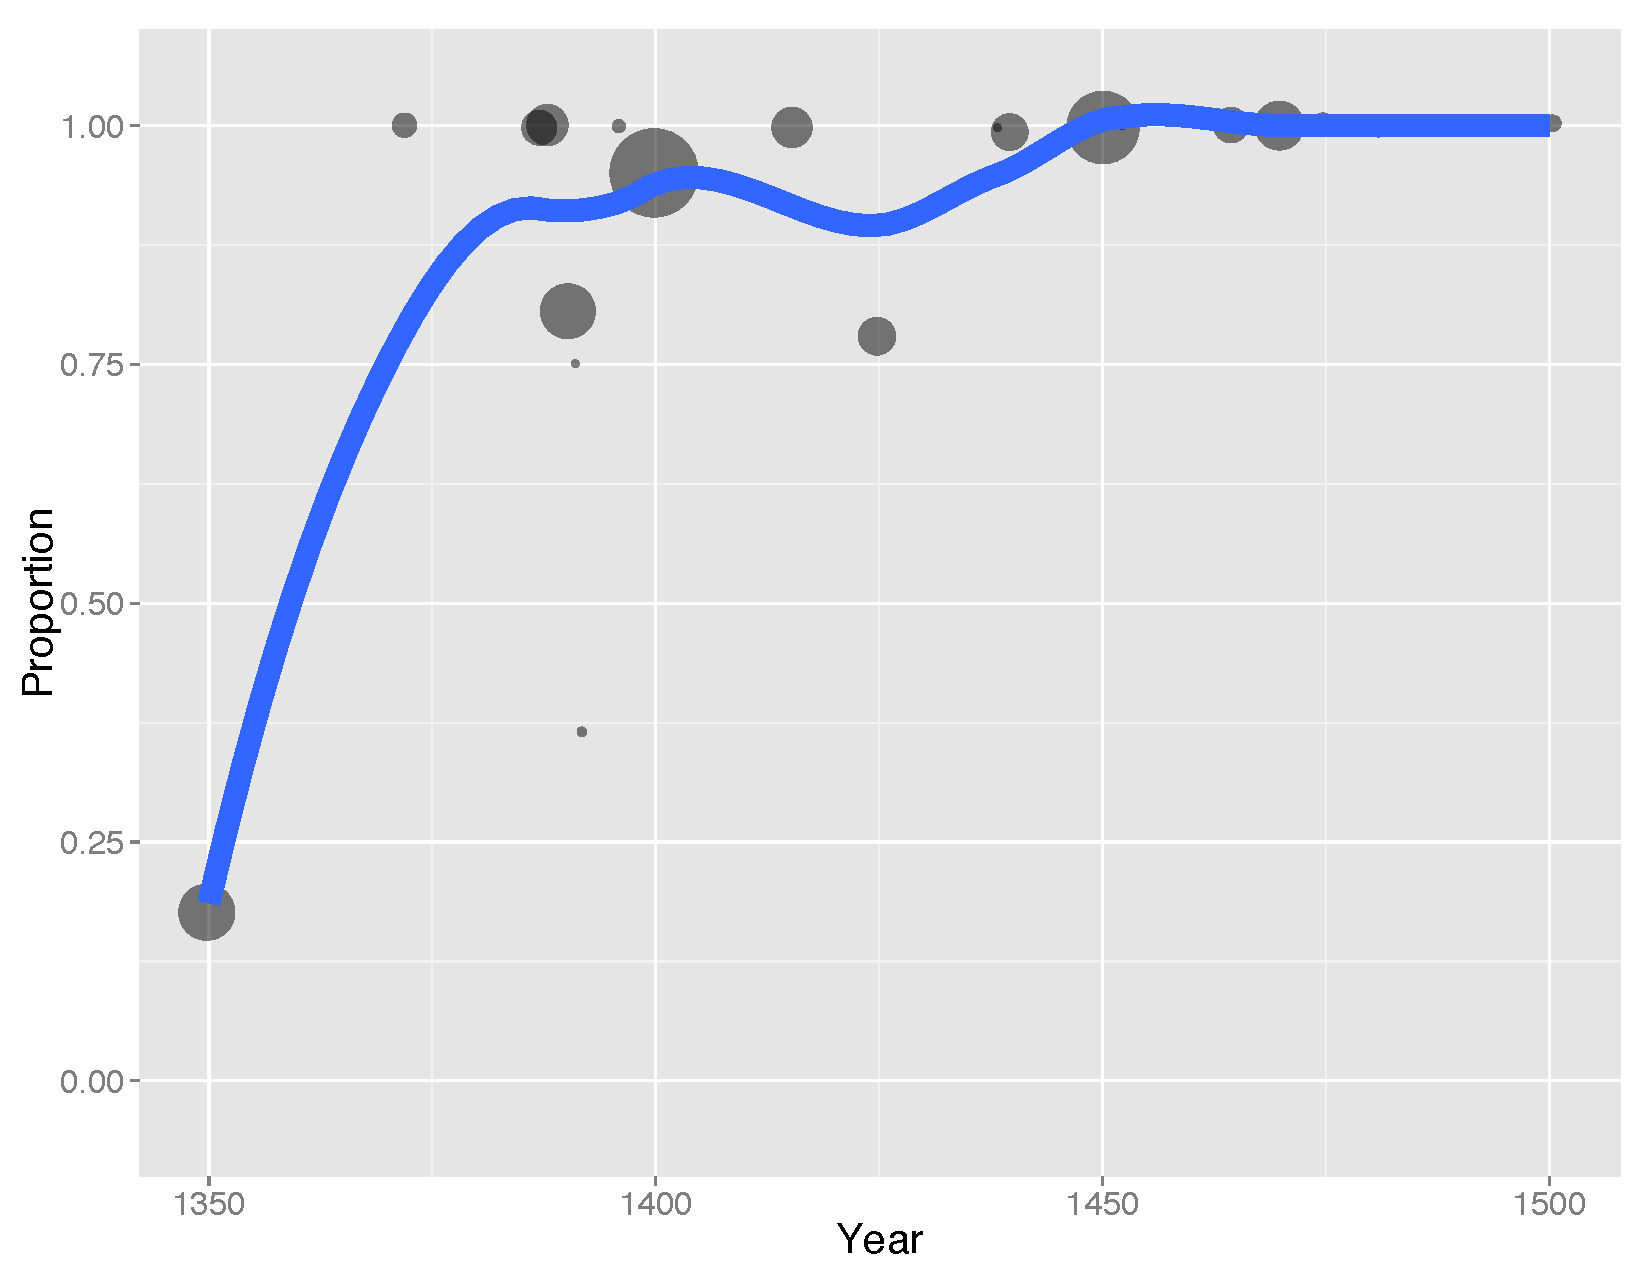
\includegraphics[width=\textwidth]{split-plot2.pdf}
\caption{Proportion of \textit{\color{green} not} versus \textit{\color{blue} ne...not} including and after 1350}
\label{split-plot2}
\end{figure}


\begin{table}[ht]
\centering
\begin{tabular}{c  l  r  l  l  l  l   r  r  l  l}
  \hline
Bins & ML$s$ & ML$\alpha$ & LRT-P & $\overline{Y}$ & $t_{FI}$ & FIT-P & $\mu$ & $\sigma_n$ & SW-P & WX-P \\ 
  \hline
  4 & 0.06728 & 1423 & 0.000086 & 0.0377 & 1.7370 & 0.1123 & 953 & 235 & 0.1218 & 0.1250 \\ 
  5 & -- & -- & -- & 0.0329 & 1.5942 & 0.1046 & 763 & 339 & 0.5138 & 0.1875 \\ 
  \hline
\end{tabular}
\caption{FIT on \textit{\color{green} not} versus \textit{\color{blue} ne...not} including and after 1350}
\label{split-table2}
\end{table}


\section{Dates}
\label{Dates}

Given that we have limited data we can't bin too finely, otherwise we run into one of two problems. Either we have an absorption event where all of the tokens are of one kind or another, or we have non-uniquely defined quantiles, we have no motivated way of splitting things up. An important question is whether these dates reflect information or are simply artifacts of uncertainty. That is, are documents dated 1225 really from 1225, or are they simply our best guess using quarter centuries?

Figure \ref{auth-plot} shows the number of documents per year. There are two important things to note. First, the documents are clustered around salient dates, roughly every quarter century. Second, we have more documents as time goes by and these are less concentrated at quarter century marks.

\begin{figure}
\centering
     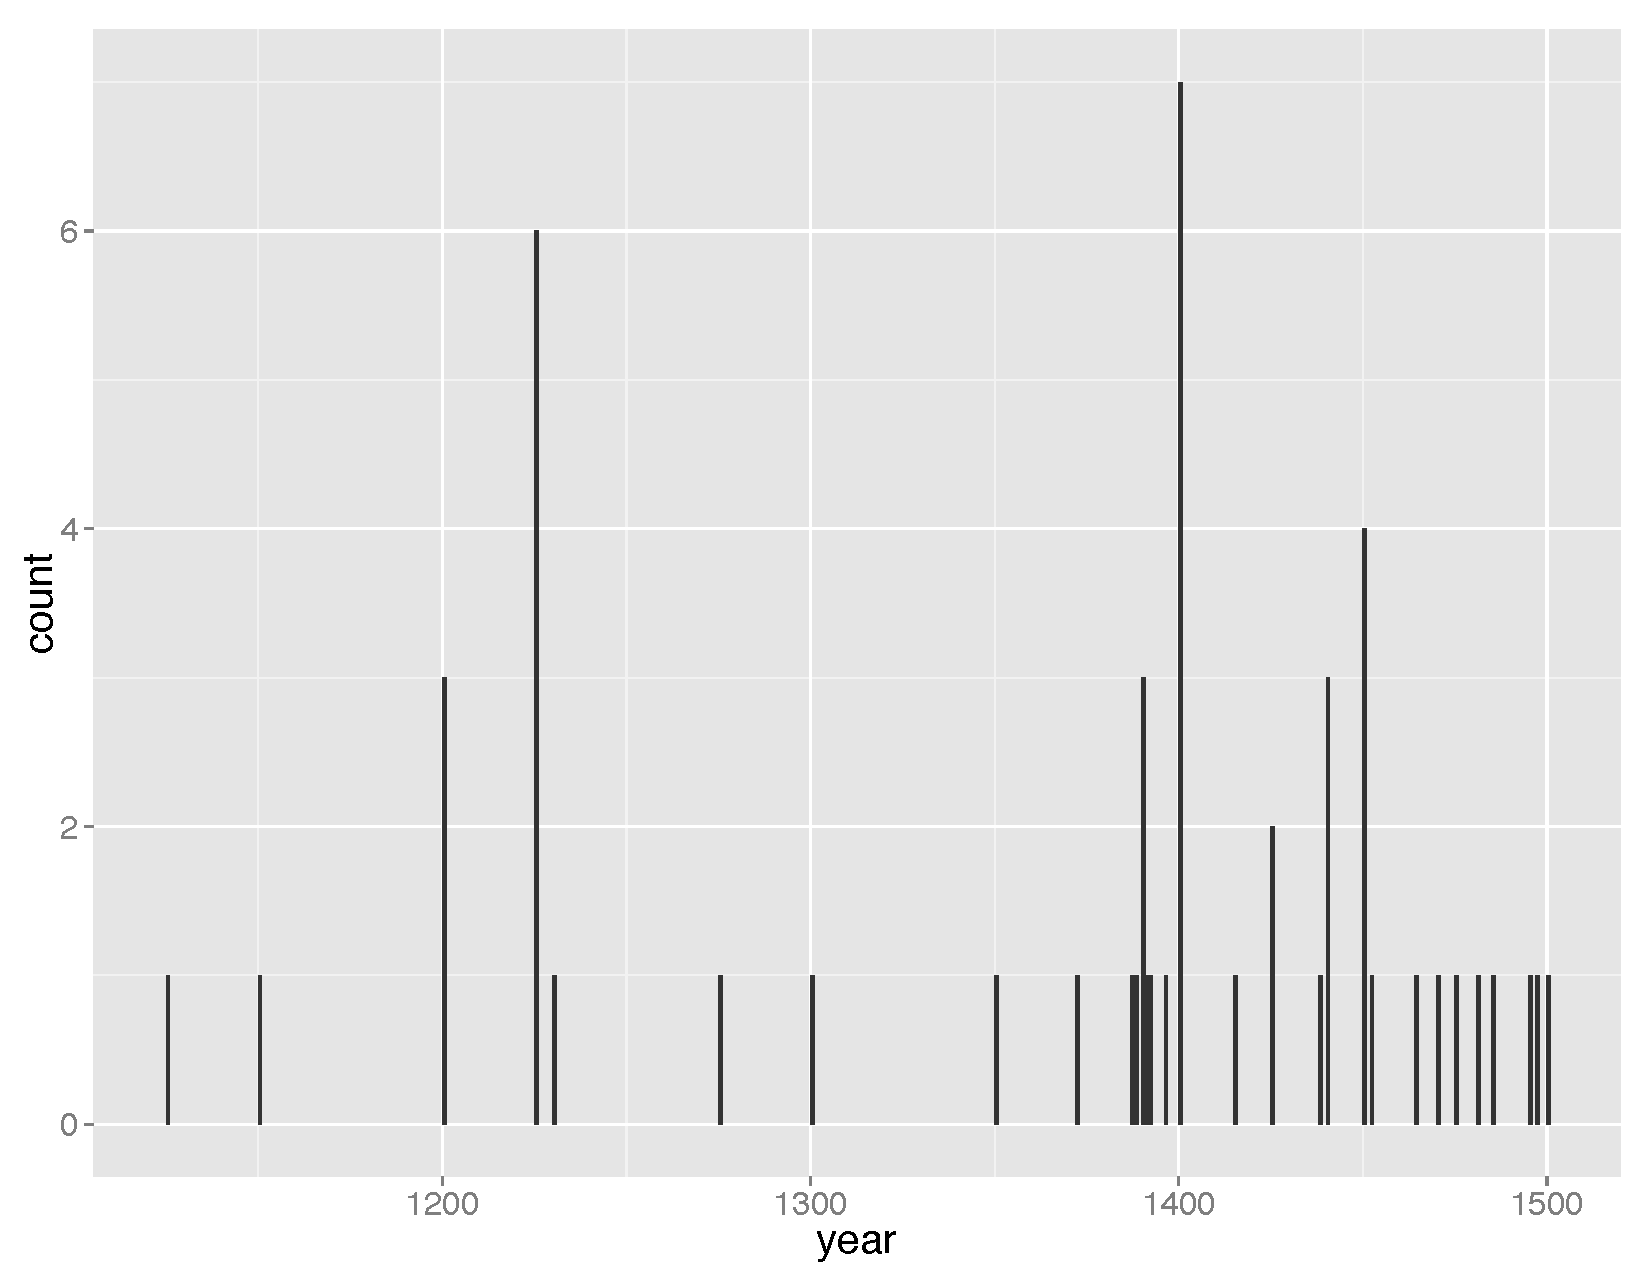
\includegraphics[width=\textwidth]{auth-plot.pdf}
\caption{Count of documents by year}
\label{auth-plot}
\end{figure}

We can try to adjust for the possibility that dates clustered around quarter century marks are artifacts rather than information by adding a small amount of noise to the date for each document. The amount of noise is uniformly distributed over $[-.5, .5 ]$. This means that documents clustered around quarter centuries will be randomly disaggregated, but no documents that are dated in unique years will be swapped in order. The upside of this is that we can simulate what would happen if we had more information about the dates of the documents.

\subsection{Lumping}

Disaggregating the data in this way allows us to bin more finely, but it doesn't shed too much more light on either transition, as we see in Tables \ref{jitter-lump-table1} and \ref{jitter-lump-table2}. For the most part, the resolution we gain from disaggregating the data is counterbalanced by the increments not being normally distributed

%\begin{figure}
%\centering
%     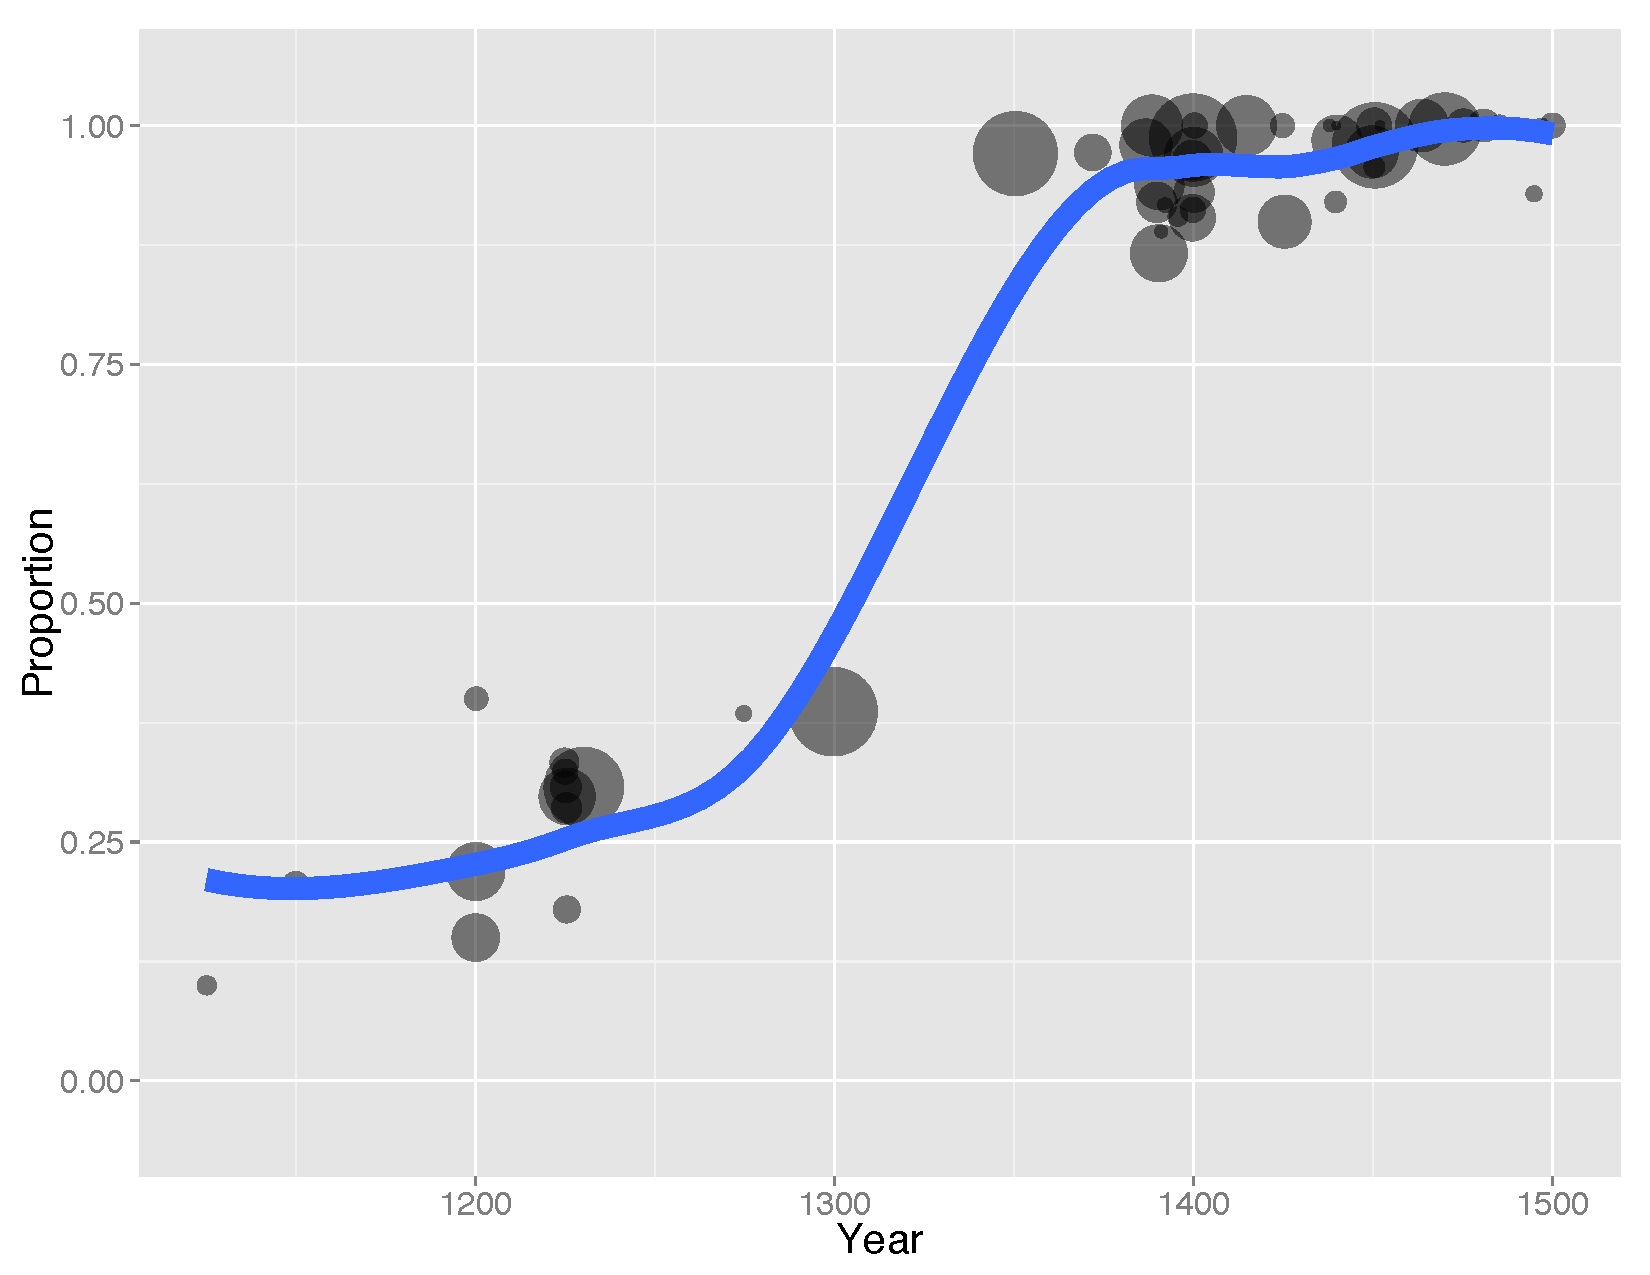
\includegraphics[width=\textwidth]{jitter-lump-plot1.pdf}
%\caption{Proportion of \textit{\color{blue} ne...not} and \textit{\color{green} not}  versus  \textit{\color{red}  ne} over time with jittered dates}
%\label{jitter-lump-plot1}
%\end{figure}

%JITTER-LUMP-FIRSTq04.out:MLS = 0.02491
%JITTER-LUMP-FIRSTq06.out:MLS = 0.01930
%JITTER-LUMP-FIRSTq07.out:MLS = 0.02590
%JITTER-LUMP-FIRSTq08.out:MLS = 0.03585
%JITTER-LUMP-FIRSTq09.out:MLS = 0.03521
%JITTER-LUMP-FIRSTq11.out:MLS = 0.02261
%
%JITTER-LUMP-FIRSTq04.out:MLALPHA = 3347
%JITTER-LUMP-FIRSTq06.out:MLALPHA = 15650
%JITTER-LUMP-FIRSTq07.out:MLALPHA = 680
%JITTER-LUMP-FIRSTq08.out:MLALPHA = 138
%JITTER-LUMP-FIRSTq09.out:MLALPHA = 47
%JITTER-LUMP-FIRSTq11.out:MLALPHA = 663
%
%JITTER-LUMP-FIRSTq04.out:CHI2P = 0.000077
%JITTER-LUMP-FIRSTq06.out:CHI2P = 0.000023
%JITTER-LUMP-FIRSTq07.out:CHI2P = 0.000033
%JITTER-LUMP-FIRSTq08.out:CHI2P = 0.000022
%JITTER-LUMP-FIRSTq09.out:CHI2P = 0.000022
%JITTER-LUMP-FIRSTq11.out:CHI2P = 0.0010


\begin{table}[ht]
\centering
\begin{tabular}{c  l  r  l  l  l  l   r  r  l  l }
  \hline
Bins & ML$s$ & ML$\alpha$ & LRT-P & $\overline{Y}$ & $t_{FI}$ & FIT-P & $\mu$ & $\sigma_n$ & SW-P  & WX-P\\ 
  \hline
  4 & 0.02491 & 3347 & 0.000077 & 0.0346 & 1.3256 & 0.1581 & 1368 & 157 & 0.1684 & 0.1250 \\ 
  5 & -- & -- & -- & 0.0320 & 2.3890 & 0.0484 & 1094 & 72 & 0.1748 & 0.0625 \\
  6 & 0.01930 & 15650 & 0.000023 & 0.0279 & 2.6530 & 0.0284 & 912 & 206 & 0.1479 & 0.0312 \\ 
  7 & 0.02590 & 680 & 0.000033 & 0.0200 & 1.4793 & 0.0996 & 781 & 206 & 0.3617 & 0.1094 \\  
  8 & 0.03585 & 138 & 0.000022 & 0.0226 & 1.4898 & 0.0934 & 684 & 84 & 0.2502 & 0.0781 \\ 
  9 & 0.03521 & 47 & 0.000022 & 0.0195 & 1.3623 & 0.1077 & 608 & 190 & 0.0009 & 0.1250 \\ 
  10 & -- & -- & -- & 0.0123 & 0.6530 & 0.2660 & 547 & 111 & 0.0397 & 0.1797 \\  
  11 & 0.02261 & 663 & 0.0010 & -- & -- & -- & -- & -- & --\\ 
  12 & -- & -- & --  &  0.0133 & 0.8299 & 0.2129 & 456 & 129 &  0.0675 & 0.0615\\
  13 & -- & -- & --  &  0.0114 & 0.7063 & 0.2473 & 420 & 127 &  0.3521 & 0.1901\\
  14 & -- & -- & --  &  0.0121 & 0.8980 & 0.1934 & 390 & 154 &  0.0828 & 0.0549\\
  15 & -- & -- & --  &  0.0072 & 0.4920 & 0.3154 & 364 & 74   &  0.1232 & 0.1478\\
   \hline
\end{tabular}
\caption{FIT on \textit{\color{red}  ne} versus \textit{\color{blue} ne...not} and \textit{\color{green} not} with jittered dates}
\label{jitter-lump-table1}
\end{table}


\begin{figure}
\centering
     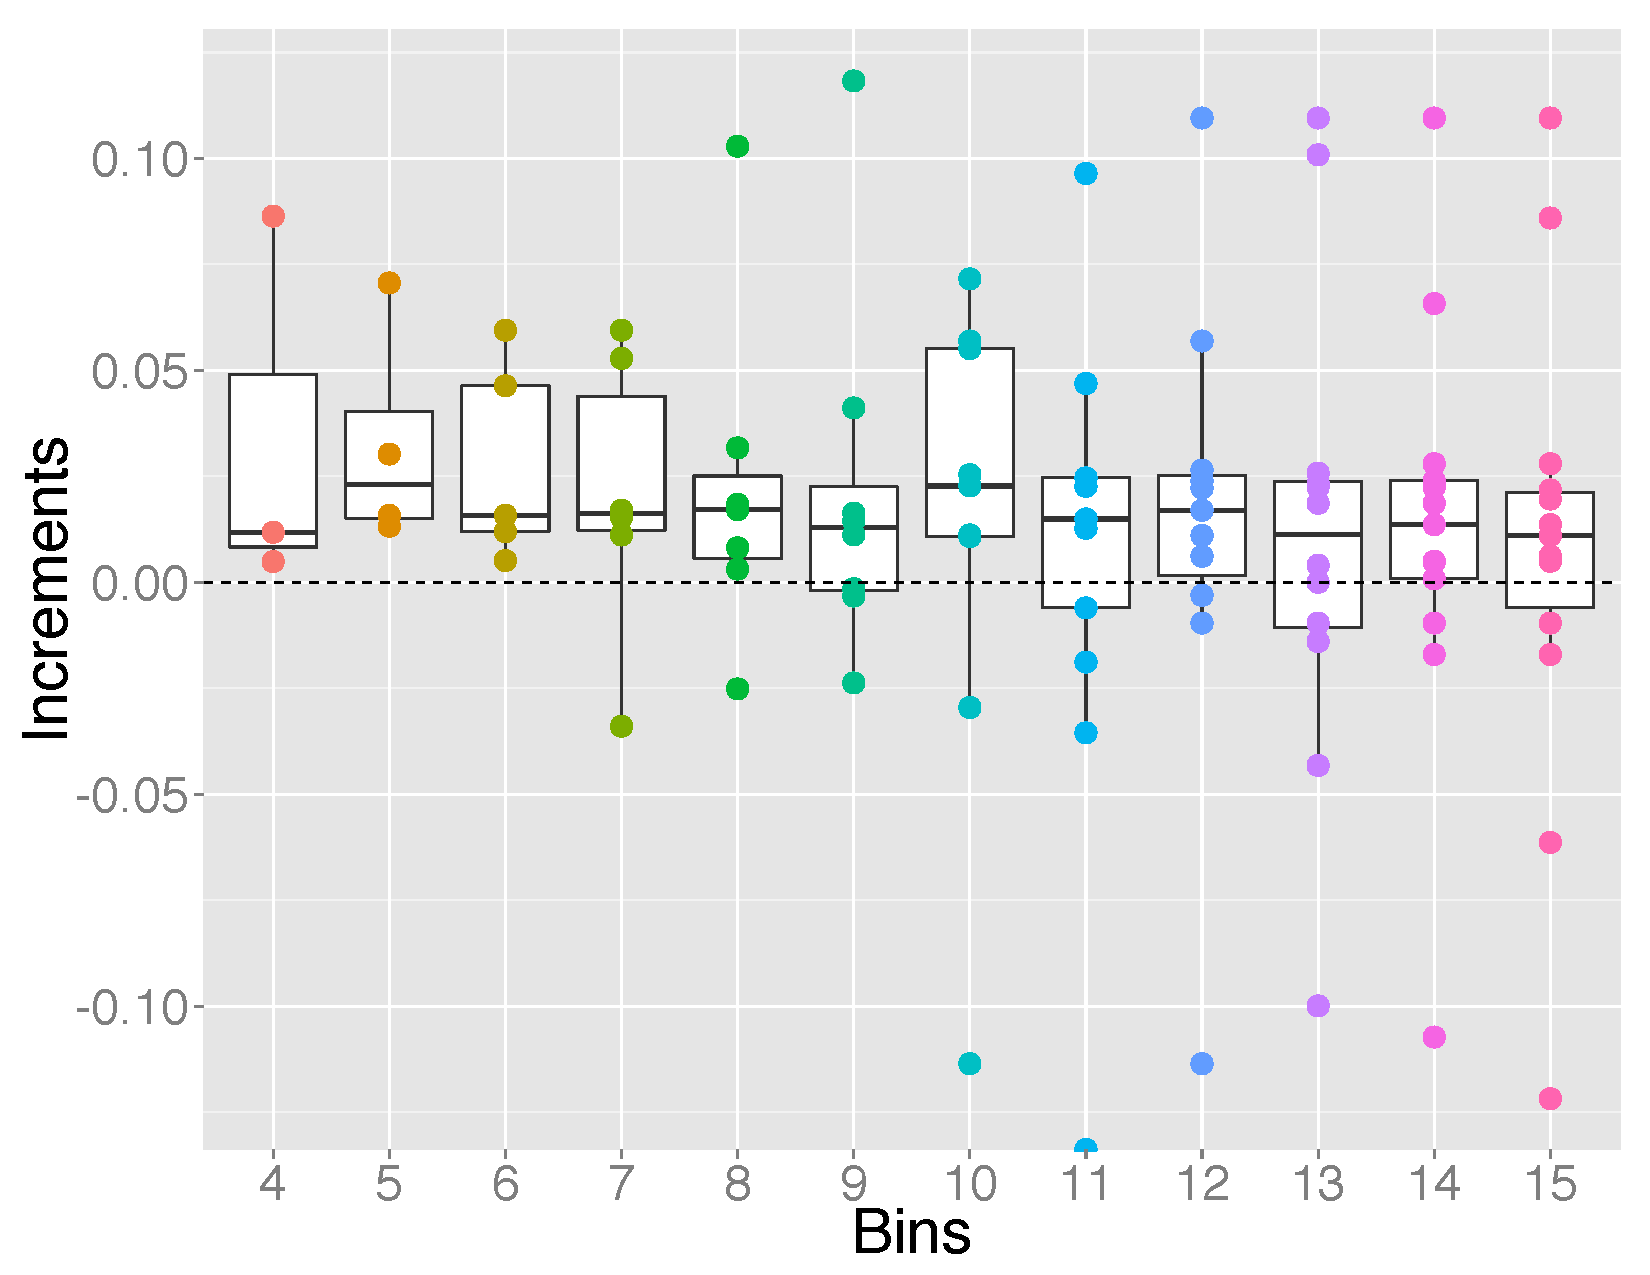
\includegraphics[width=\textwidth]{jitter-lump-first-increments.pdf}
\caption{Distribution of increments for  comparison of \textit{\color{blue} ne...not} and \textit{\color{green} not}  versus  \textit{\color{red}  ne} over time with jittered dates}
\label{jitter-lump-first-increments}
\end{figure}




%\begin{figure}
%\centering
%     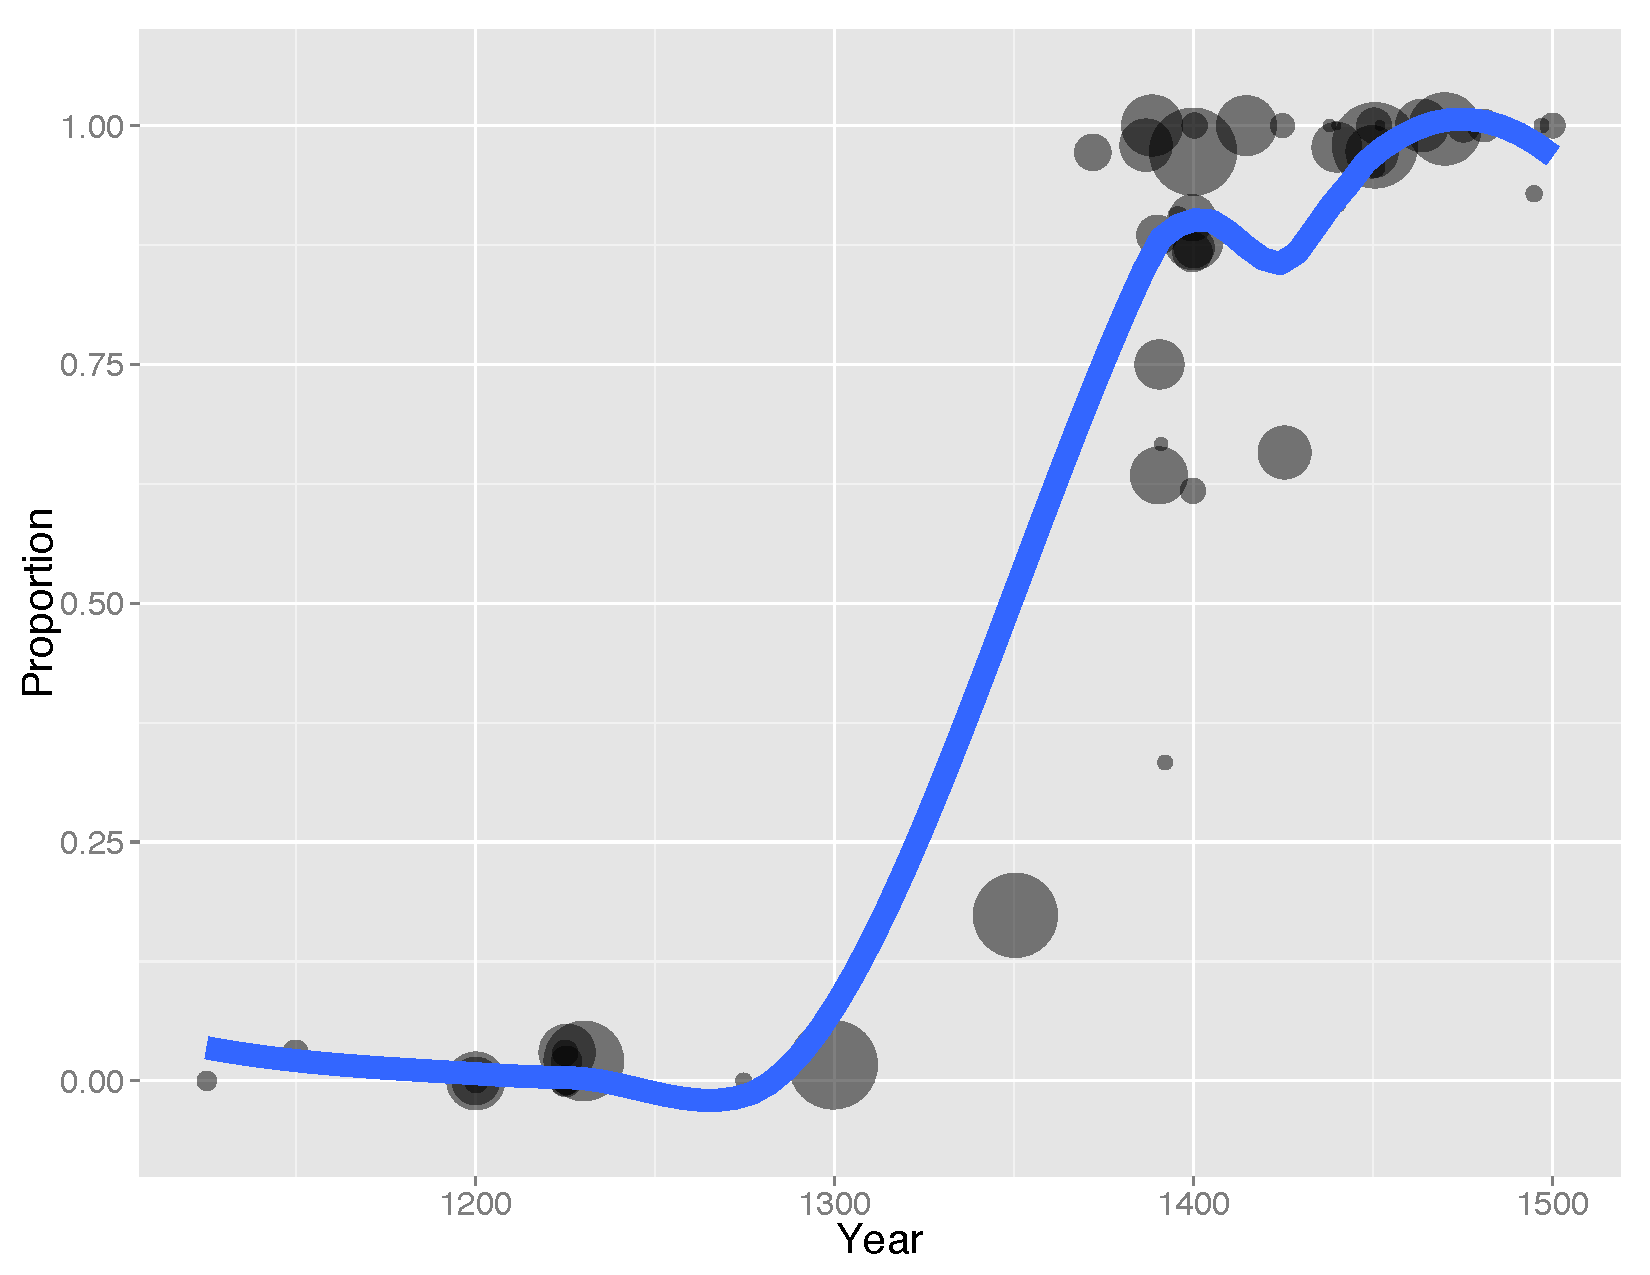
\includegraphics[width=\textwidth]{jitter-lump-plot2.pdf}
%\caption{Proportion of \textit{\color{green} not} versus \textit{\color{red}  ne} and \textit{\color{blue} ne...not} over time with jittered dates}
%\label{jitter-lump-plot2}
%\end{figure}

%JITTER-LUMP-SECONDq07.out:MLS = 0.03829
%JITTER-LUMP-SECONDq09.out:MLS = 0.03523
%JITTER-LUMP-SECONDq10.out:MLS = 0.03250
%JITTER-LUMP-SECONDq13.out:MLS = 0.07745
%JITTER-LUMP-SECONDq15.out:MLS = 0.00458
%
%JITTER-LUMP-SECONDq07.out:MLALPHA = 112
%JITTER-LUMP-SECONDq09.out:MLALPHA = 224
%JITTER-LUMP-SECONDq10.out:MLALPHA = 102
%JITTER-LUMP-SECONDq13.out:MLALPHA = $\infty$
%JITTER-LUMP-SECONDq15.out:MLALPHA = 9
%
%JITTER-LUMP-SECONDq07.out:CHI2P = 0.00028
%JITTER-LUMP-SECONDq09.out:CHI2P = 0.000050
%JITTER-LUMP-SECONDq10.out:CHI2P = 0.00090
%JITTER-LUMP-SECONDq13.out:CHI2P = --
%JITTER-LUMP-SECONDq15.out:CHI2P = --


\begin{table}[ht]
\centering
\begin{tabular}{c  l  r  l  l  l  l   r  r  l  l}
  \hline
Bins & ML$s$ & ML$\alpha$ & LRT-P & $\overline{Y}$ & $t_{FI}$ & FIT-P & $\mu$ & $\sigma_n$ & SW-P  & WX-P\\ 
  \hline
  4 & -- & -- & -- & 0.1315 & 1.3848 & 0.1502 & 1368 & 145 & 0.1135 & 0.1250 \\ 
  5 & -- & -- & -- & 0.0812 & 1.9173 & 0.0755 & 1094 & 77 & 0.1333 & 0.0625\\ 
  6 & -- & -- & -- & 0.0621 & 1.7023 & 0.0820 & 912 & 164 & 0.0065 & 0.0312\\ 
  7 & 0.03829 & 112 & 0.00028 & 0.0428 & 0.9306 & 0.1974 & 781 & 204 & 0.2285 & 0.1563\\ 
  8 & -- & -- & -- & 0.0656 & 1.7613 & 0.0643 & 684 & 78 & 0.0507 & 0.0391\\ 
  9 & 0.03523 & 224 & 0.000050 & 0.0463 & 1.6840 & 0.0680 & 608 & 193 & 0.0633 & 0.0547\\ 
  10 & 0.03250 & 102 & 0.00090 & 0.0137 & 0.2563 & 0.4021 & 547 & 128 & 0.0735 & 0.1504\\  
  11 & -- & -- & -- & -- & -- & -- & -- & -- & -- & --\\  
  12 & -- & -- & -- & 0.0120 & 0.2760 & 0.3940 & 456 & 129 & 0.0674 & 0.2065\\
  13 & 0.07745 & $\infty$ & -- & 0.0274 & 0.9516 & 0.1808 & 420 & 127 & 0.9002 & 0.2592\\
  14 & -- & -- & -- & 0.0149 & 0.3916 & 0.3511 & 390 & 154 & 0.0614 & 0.2274\\
  15 & 0.00458 & 9 & -- & 0.0042 & 0.1146 & 0.4552 & 364 & 74   & 0.0273 & 0.1629\\
  \hline
  \end{tabular}
\caption{FIT on \textit{\color{red}  ne} and \textit{\color{blue} ne...not} versus  \textit{\color{green} not} with jittered dates}
\label{jitter-lump-table2}
\end{table}

\begin{figure}
\centering
     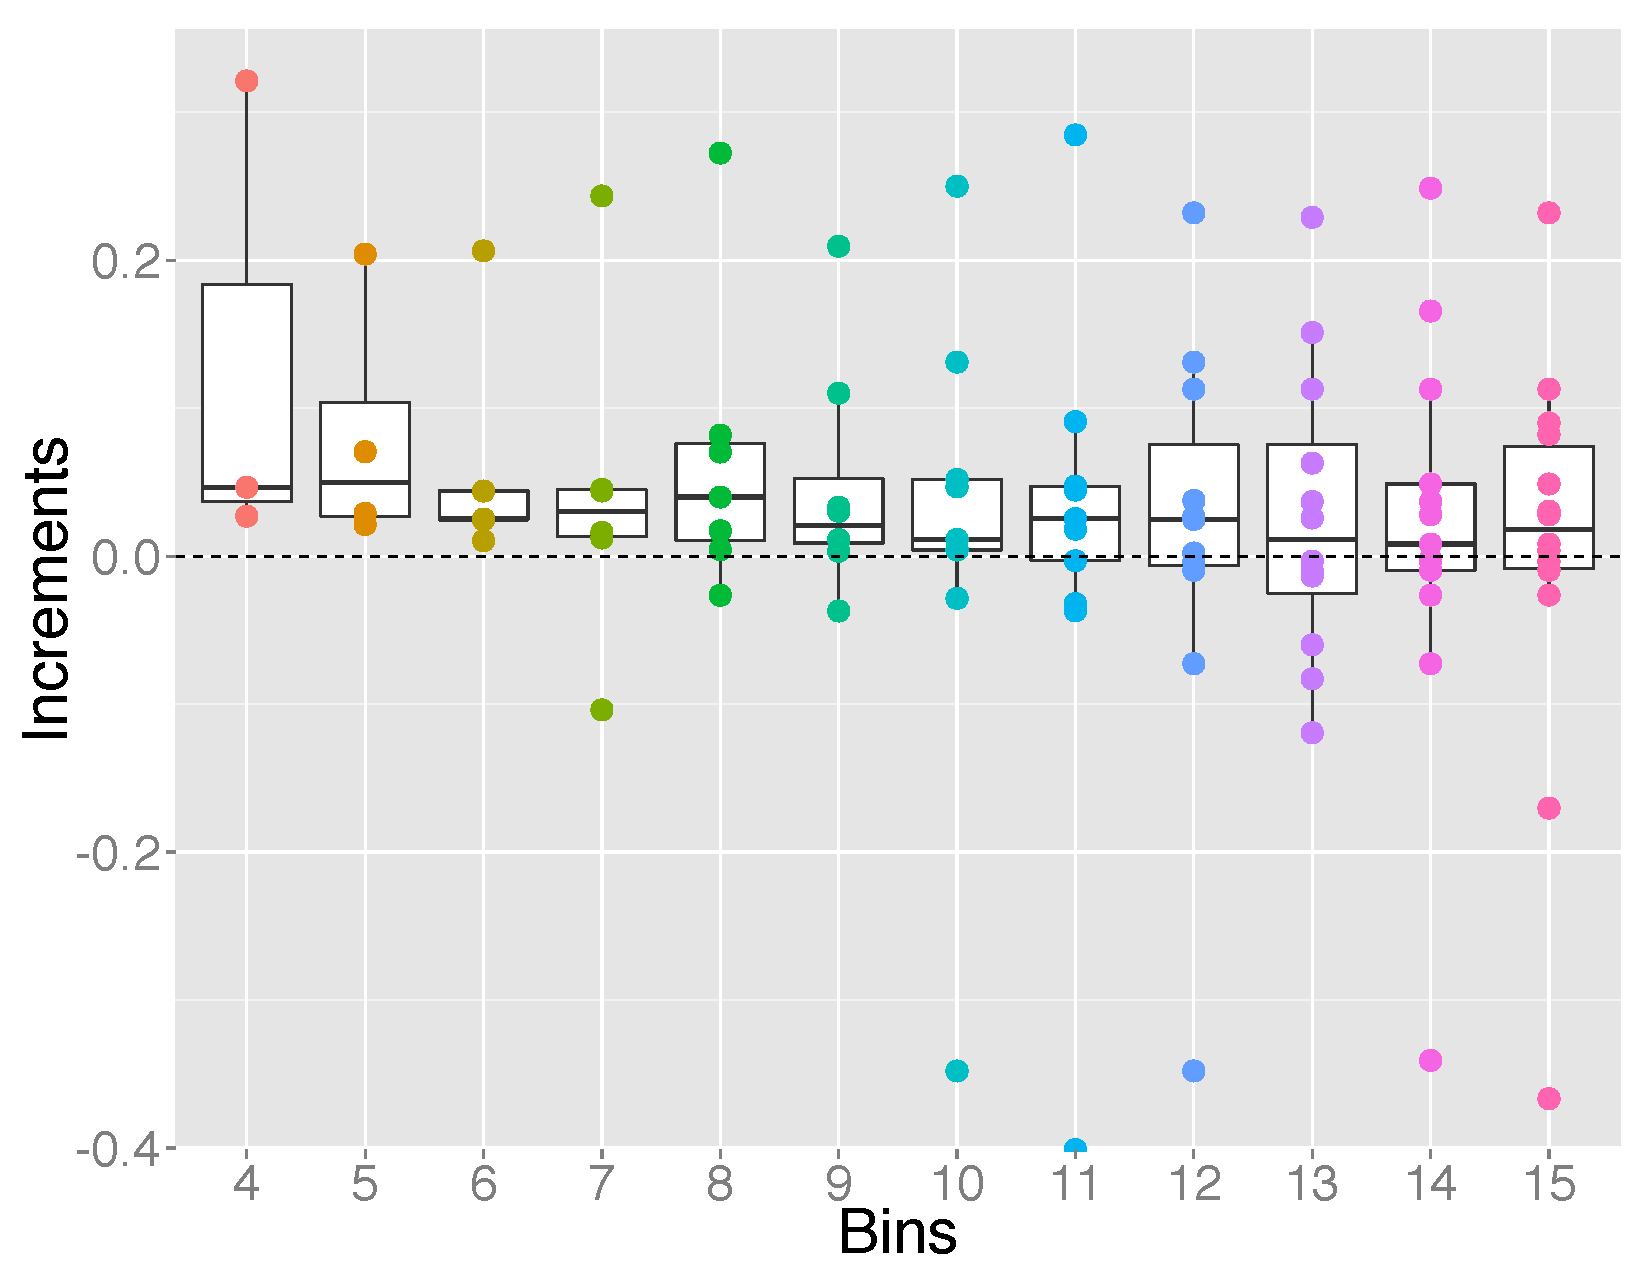
\includegraphics[width=\textwidth]{jitter-lump-second-increments.pdf}
\caption{Distribution of increments for  comparison of \textit{\color{red}  ne} and \textit{\color{blue} ne...not} versus  \textit{\color{green} not} over time with jittered dates}
\label{jitter-lump-second-increments}
\end{figure}


\subsection{Splitting}

Again, disaggregating the data in this way allows us to bin more finely, but only in the case of the second transition. However, we still don't find sufficient evidence to reject the null hypothesis of drift, as we can see in Tables \ref{jitter-split-table1} and \ref{jitter-split-table2}.

 
 
\begin{figure}
\centering
     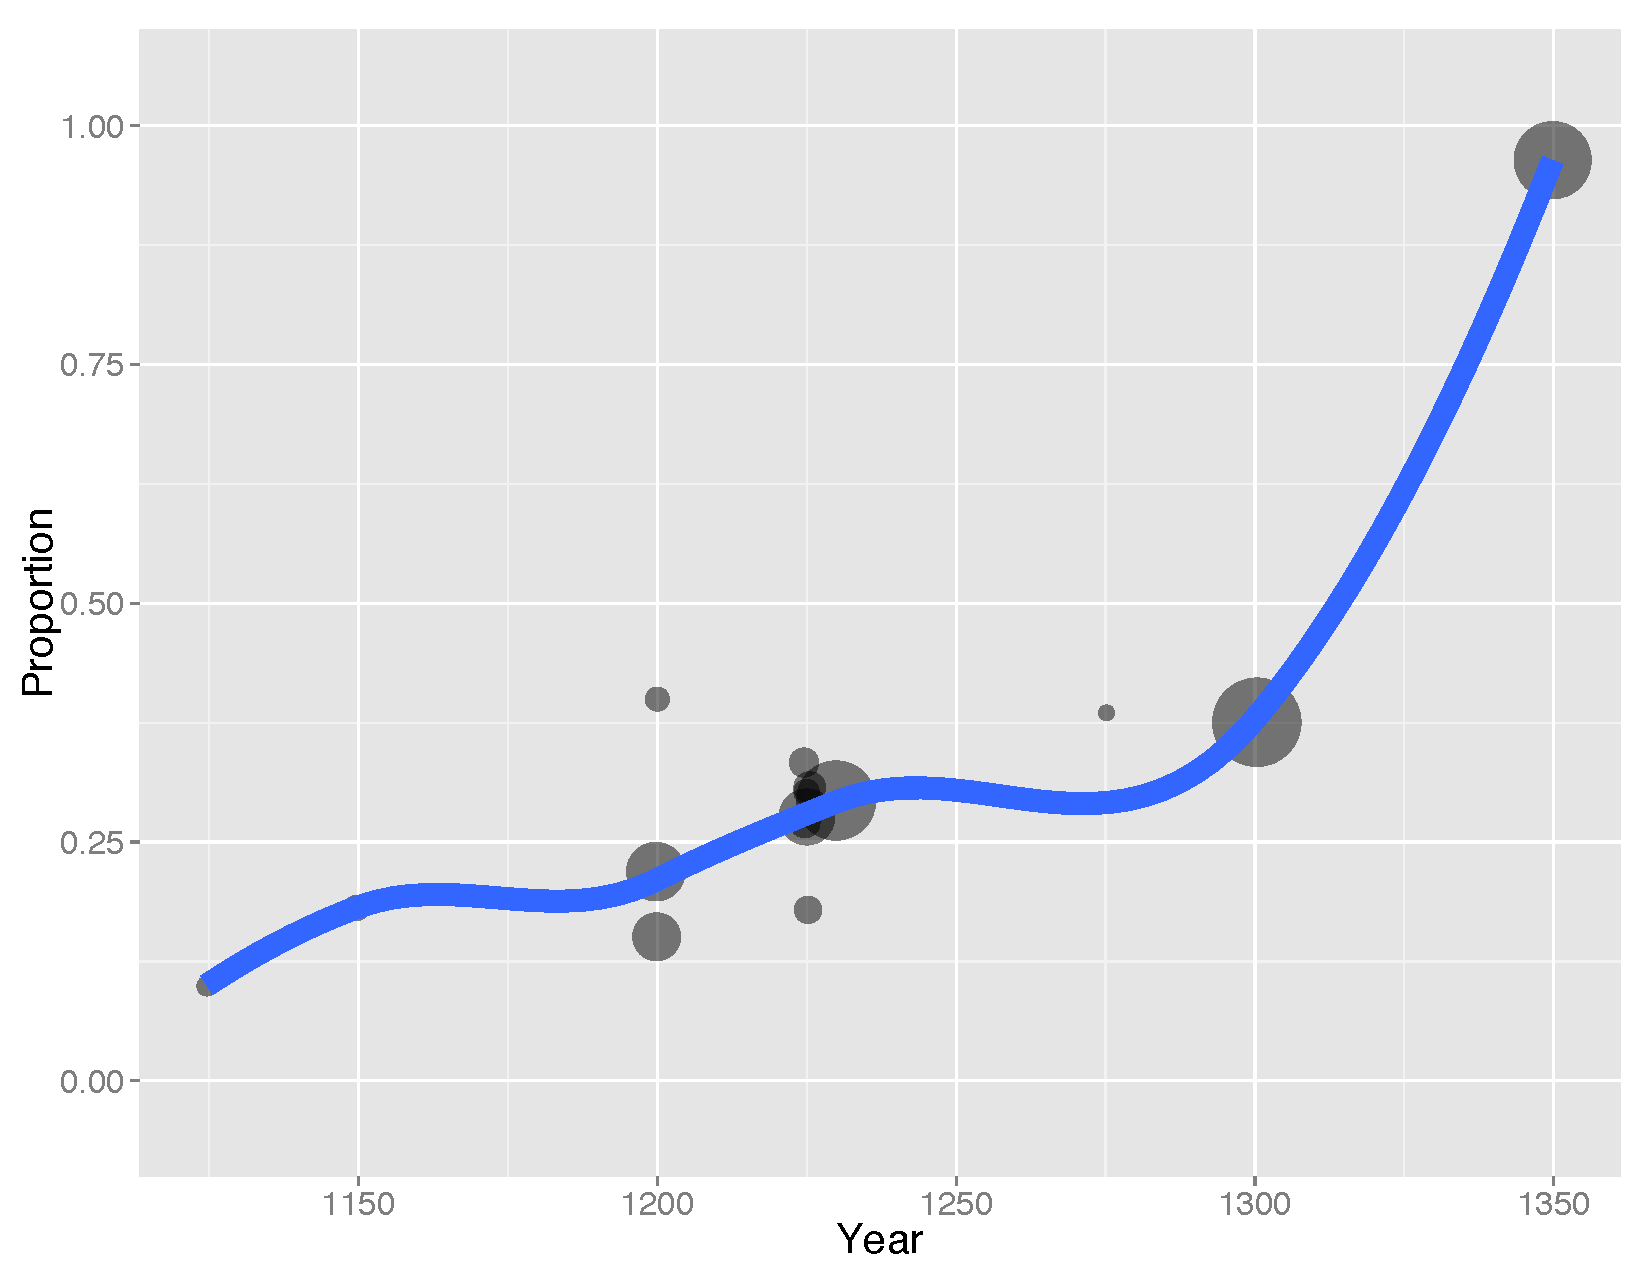
\includegraphics[width=\textwidth]{jitter-split-plot1.pdf}
\caption{Proportion of \textit{\color{blue} ne...not} and \textit{\color{green} not}  versus  \textit{\color{red}  ne} over time with jittered dates}
\label{jitter-split-plot1}
\end{figure}

%JITTER-SPLIT-FIRSTq04.out:MLS = 0.02697
%JITTER-SPLIT-FIRSTq05.out:MLS = 0.01140
%
%JITTER-SPLIT-FIRSTq04.out:MLALPHA = 284
%JITTER-SPLIT-FIRSTq05.out:MLALPHA = 304
%
%JITTER-SPLIT-FIRSTq04.out:CHI2P = 0.092
%JITTER-SPLIT-FIRSTq05.out:CHI2P = 0.23

\begin{table}[ht]
\centering
\begin{tabular}{c  l  r  l  l  l  l   r  r  l  }
  \hline
Bins & ML$s$ & ML$\alpha$ & LRT-P & $\overline{Y}$ & $t_{FI}$ & FIT-P & $\mu$ & $\sigma_n$ & SW-P \\ 
  \hline
  4 & 0.02697 & 284 & 0.092 & 0.0497 & 1.6164 & 0.1237 & 454 & 126 & 0.1687 \\ 
  5 & 0.01140 & 304 & 0.23 & 0.0458 & 1.4588 & 0.1204 & 363 & 38 & 0.0248 \\    \hline
\end{tabular}
\caption{FIT on \textit{\color{red}  ne} versus \textit{\color{blue} ne...not} with jittered dates}
\label{jitter-split-table1}
\end{table}


\begin{figure}
\centering
     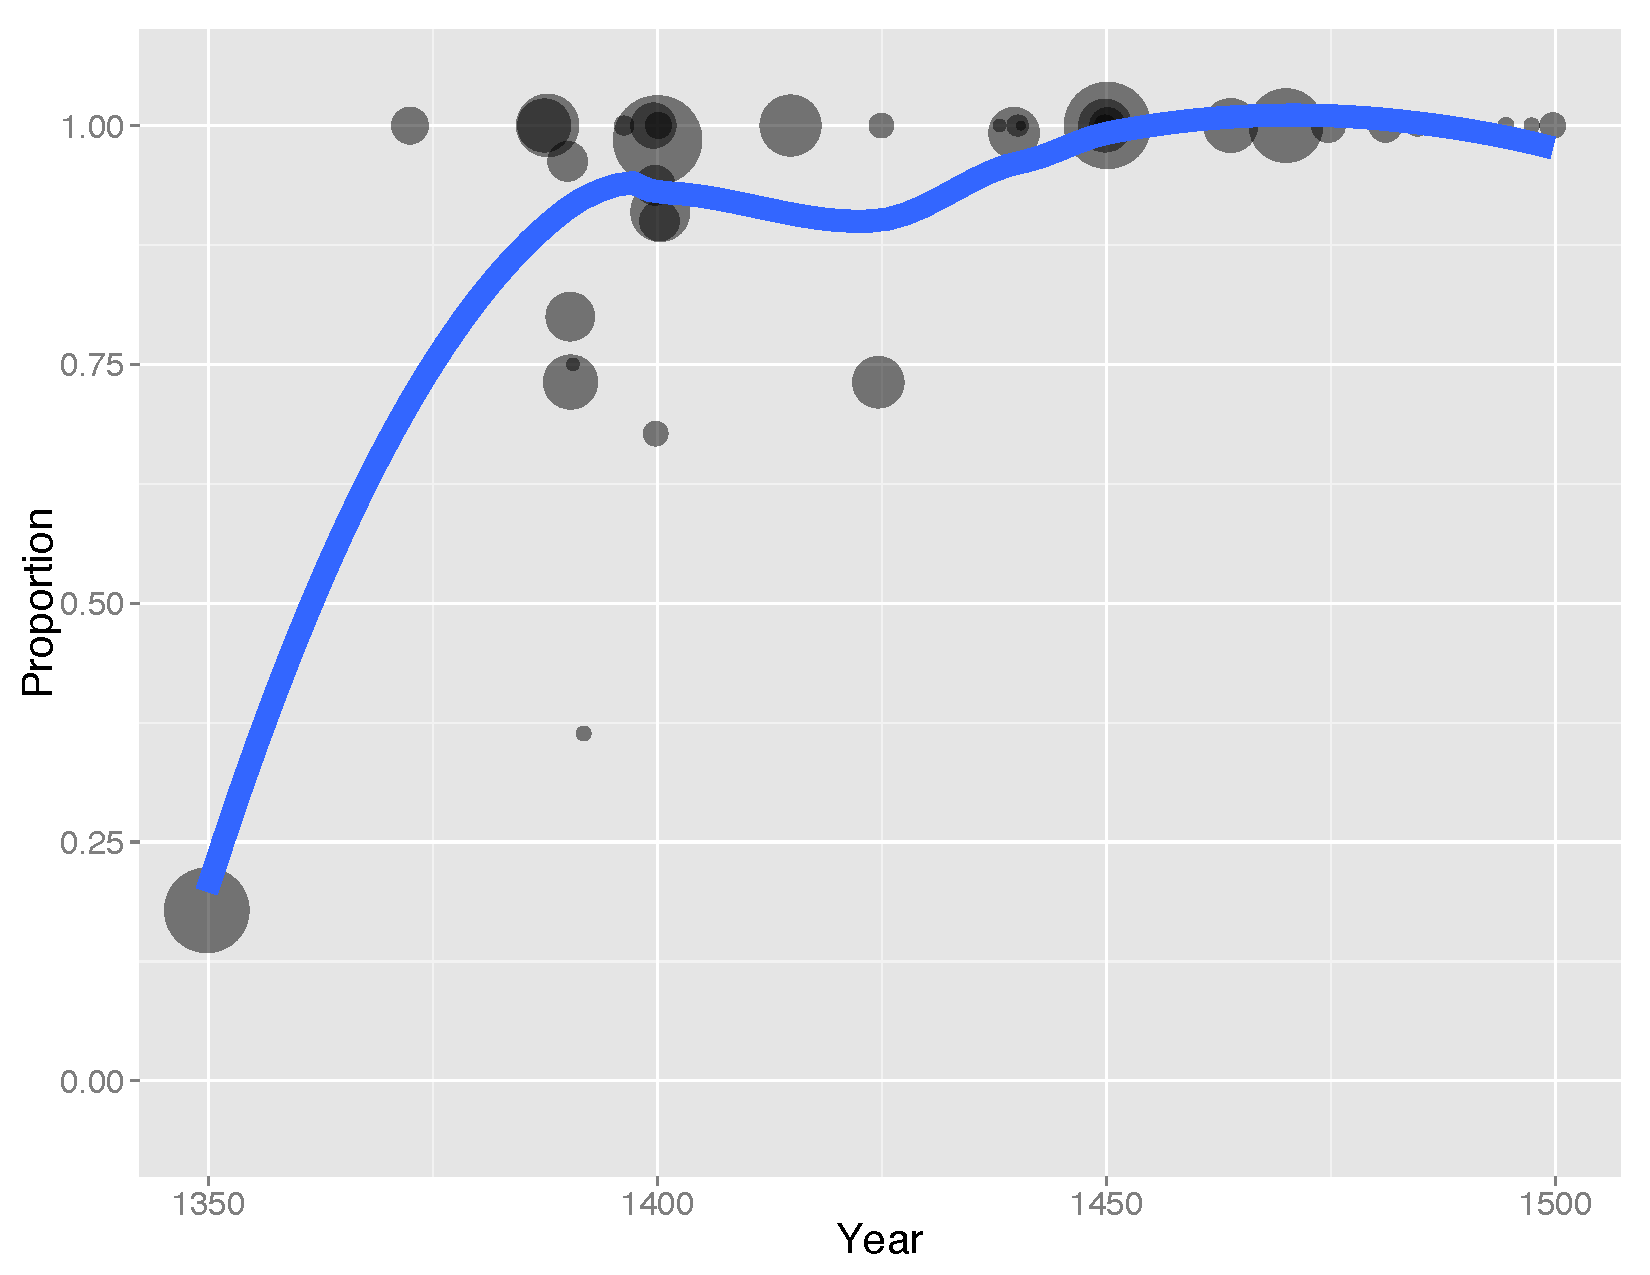
\includegraphics[width=\textwidth]{jitter-split-plot2.pdf}
\caption{Proportion of \textit{\color{green} not} versus \textit{\color{red}  ne} and \textit{\color{blue} ne...not} over time with jittered dates}
\label{jitter-split-plot2}
\end{figure}

%JITTER-SPLIT-SECONDq04.out:MLS = 0.05791
%JITTER-SPLIT-SECONDq05.out:MLS = 0.11907
%
%JITTER-SPLIT-SECONDq04.out:MLALPHA = 15660
%JITTER-SPLIT-SECONDq05.out:MLALPHA = 24
%
%JITTER-SPLIT-SECONDq04.out:CHI2P = 0.000045
%JITTER-SPLIT-SECONDq05.out:CHI2P = 0.000068
%

\begin{table}[ht]
\centering
\begin{tabular}{c  l  r  l  l  l  l   r  r  l  }
  \hline
Bins & ML$s$ & ML$\alpha$ & LRT-P & $\overline{Y}$ & $t_{FI}$ & FIT-P & $\mu$ & $\sigma_n$ & SW-P \\ 
  \hline
  4 & 0.05791 & 15660 & 0.000045 & 0.0391 & 2.2066 & 0.0790 & 953 & 181 & 0.1385 \\ 
  5 & 0.11907 & 24 & 0.000068 & 0.0335 & 1.6935 & 0.0945 & 763 & 144 & 0.4040 \\ 
  6 & -- & -- & -- & -- & 2.1307 & 0.0615 & 635 & 100 & 0.2593 \\ 
  7 & -- & -- & -- & -- & 1.6475 & 0.0874 & 545 & 65 & 0.6893 \\ 
  8 & -- & -- & -- & -- & 1.0583 & 0.1692 & 476 & 211 & 0.0682 \\ 
  9 & -- & -- & -- & -- & -0.0420 & 0.5159 & 423 & 111 & 0.5804 \\   \hline
  \end{tabular}
\caption{FIT on \textit{\color{blue} ne...not} versus  \textit{\color{green} not} with jittered dates}
\label{jitter-split-table2}
\end{table}


%\section{Introduction}
%
%Here we'll compare different ways of binning time series data to test for drifts versus selection. The goal will be to motivate  a particular method for binning the data. We'll compare fixed- and variable-width bins for the $\chi^2$ likelihood ratio test (LRT) and the fitness increment test (FIT). Before moving on to the data and the particular methods, we note two sets of constraints on how we bin the data which are motivated by the results in \cite{feder-etal2014}. 
%
%The first set of constraints are \textbf{theoretical} and have to do with what we are calculating. For example, to jointly estimate the maximum likelihood population size and selection coefficient for the LRT we need at least three data points and thus at least three bins (p.511). Likewise, to perform the FIT we need at least two increments to compute the test statistic and thus at least three bins (p.512). In the opposite direction, we can't bin the data too finely because the fitness increment test is only appropriate if no absorption event occurs prior to the last bin (p.516). No document without variation between the forms can constitute its own bin, unless it happens to be the last document. Additionally, we cannot have more bins than there are uniquely-dated documents. Otherwise we'll end up with empty bins, which will render the FIT undefined. Finally, the Gaussian approximation of the diffusion process rests on the assumption of normality both in the movement of allele frequency and the distribution 
%of the rescaled fitness increments. We'll need at least three increments, and thus four bins to test for normality.
%
%The second set of constraints are \textbf{practical} and have to do with the power of the tests we are calculating, in particular, the power of the FIT. When samples are drawn at equal intervals, the power of the FIT grows weakly with and increase in the number of sampled time points (p.514, Figure 2), which is reproduced here in Figure \ref{power}. This suggests that the more bins we have the better. However, with noisy sampling at equally-spaced intervals, the statistical power of the FIT decreases with fewer samples drawn (p.517, Figure 5), which is reproduced in Figure \ref{power-sample}. Given that historical data are limited, this suggests that the fewer bins we have the better. While historical documents are not ``sampled'' at equal intervals, this second set of constraints suggests that we want a balance between how many bins we have and the number of data points per bin that we have. 
%
%\begin{figure}
%\centering
%     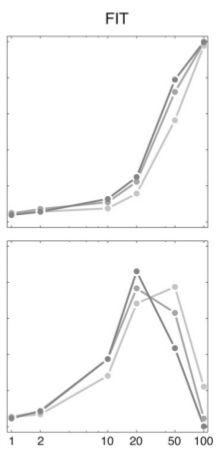
\includegraphics[width=3in]{power.png}
%\caption{Power of FIT for $L = 5, 10, 50$ for various levels of selection pressure $Ns$}
%\label{power}
%\end{figure}
%
%\begin{figure}
%\centering
%     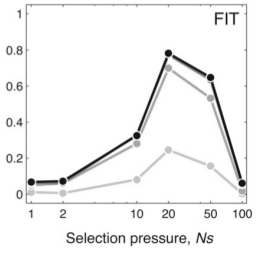
\includegraphics[width=3in]{power-sample.png}
%\caption{Power of FIT for $L = 10$ for various levels of selection pressure $Ns$ with samples of size $n = 100, 1000, 10000$}
%\label{power-sample}
%\end{figure}
%
%
%
%Our goal will be to find a method of binning that abides by the first set of constraints, while striking a balance between the competing demands of the second set of constraints. We begin in Section \ref{do-support} with a  brief overview of the \emph{do}-support data and compare results for fixed- and variable-width bins.
%
%\section{\emph{do}-support}
%\label{do-support}
%
%The general trajectory of the change in \emph{do}-support is shown in Figure \ref{do-support-sub}. In what follows, we'll pool the data across contexts, leaving investigations of individual contexts for future exploration.
%
%\begin{figure}
%\centering
%     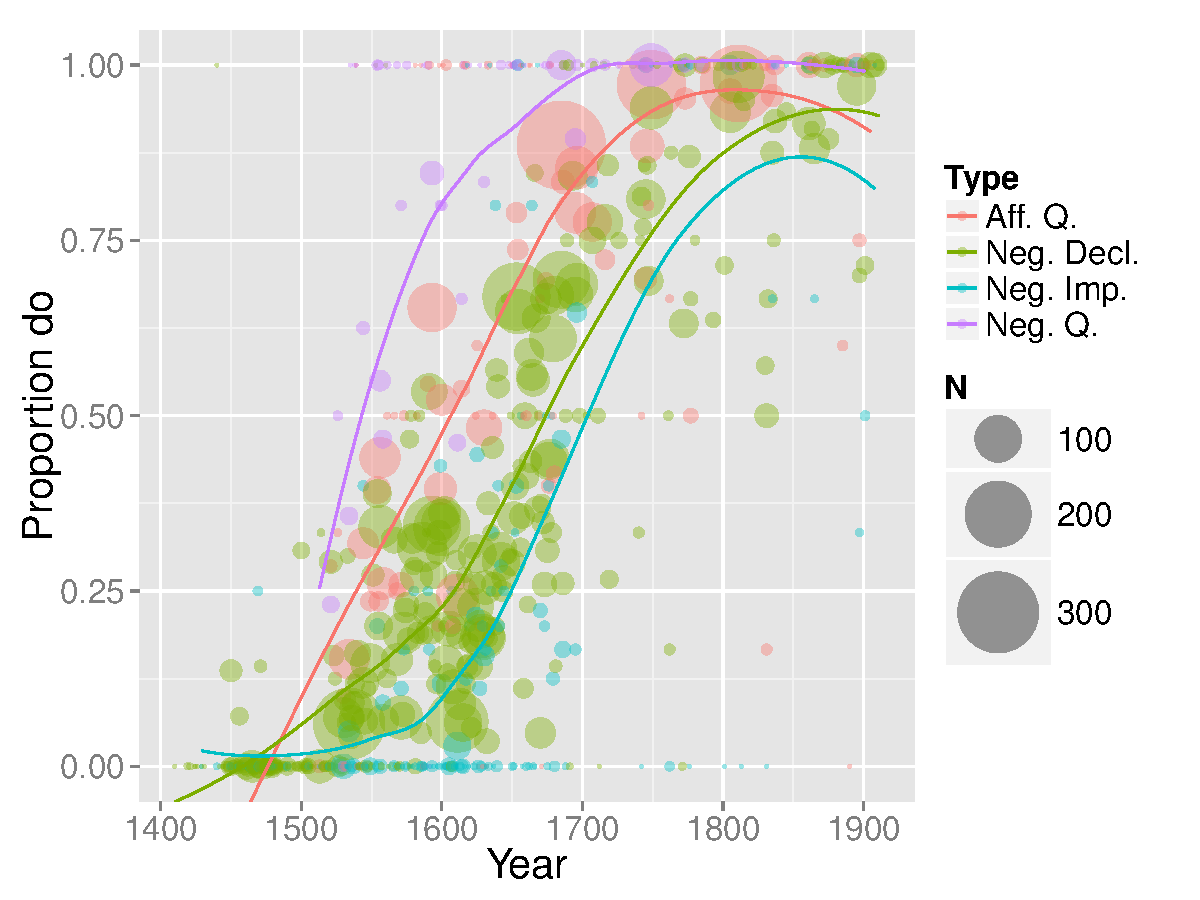
\includegraphics[width=\textwidth]{do-support-drift.pdf}
%\caption{Proportion of \emph{do}-support in coherent contexts}
%\label{do-support-sub}
%\end{figure}
%
%In what follows, we'll include all tokens from the very instance of \emph{do}-support onwards. The first instance occurs in 1440. Originally, I'd used only those tokens from 1500 to 1900, to allow an easy comparison between fixed-width bins across contexts (e.g. negative declaratives versus negative imperatives, etc.). However, since we are not examining or comparing across contexts, or using fixed-width bins, it makes far more sense to include as much data as possible.  In fact, doing so allows us to add around seven hundred more tokens to our analysis.  In data from 1440 on, we have a little more than 11,000 tokens with 307 years represented, as well as roughly 2,500 individual documents by 600 authors.\footnote{The estimate of authors slightly low. Around 50 authors are labeled together.}
%
%We can get a general sense of the distribution of tokens over time and the difference between fixed- and variable-width bins in Figure \ref{do-compare-all}. The count of tokens per bin is shown for both fixed-width (gray) and variable-width bins (white). The variable-width bins are quantiles, where the number of tokens is as close to even across bins as possible.\footnote{There are several algorithms for calculating quantiles. For now, I've simply used the default, but this is something to explored. This might be particularly relevant when the quantiles are not uniquely defined by a particular algorithm.} In the upper-left, where the number of bins $n=4$, we see that the fixed-width bins vary rather widely, whereas the variable-width quantiles quite a bit less, exactly as we would expect.
%
%\begin{figure}
%\centering
%     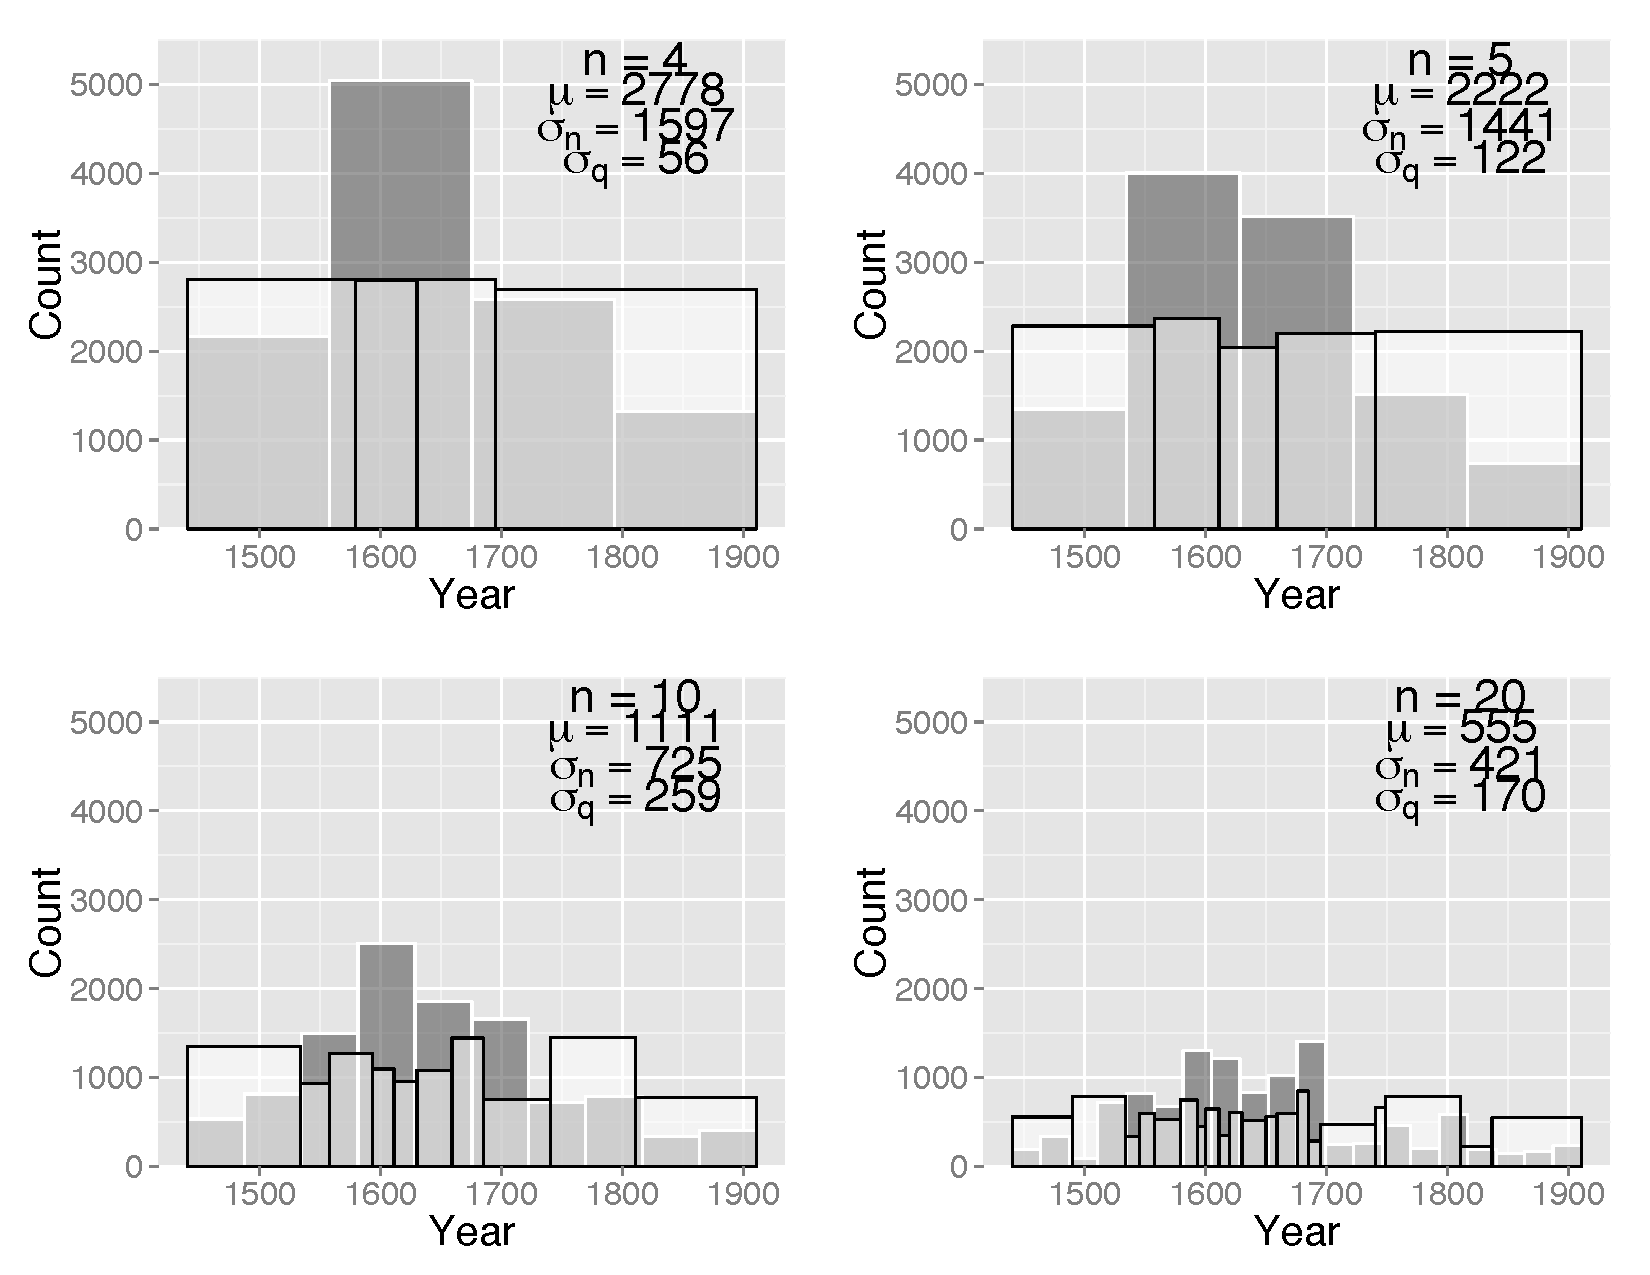
\includegraphics[width=\textwidth]{do-compare-all.pdf}
%\caption{Count of tokens per bin for fixed- (gray) and variable width bins (white) for $n = 4,5,10,20$}
%\label{do-compare-all}
%\end{figure}
%
%Figure \ref{do-compare-all} also shows the mean number of tokens  per bin $\mu$, the standard deviation of the fixed-width bins $\sigma_n$, and the standard deviation of the variable-width bins $\sigma_q$. As the number of bins increases, the average number of tokens per bin decreases, the variance of the number of tokens per fixed-width bins decreases, and the variance of the number of tokens per variable-width bins increases.
%
%
%\subsection{Fixed-Width Bins}
%
%We start with all of the data pooled together and bin from four to an increasing number of bins. Given that there are several thousand tokens of potential instances of \emph{do}-support, we could reasonably partition the data rather finely. Table \ref{do-n-bin-all} gives the results for different numbers of bins.
%
%We report the results for the $\chi^2$  LRT, including the output from \emph{tsinfer} where possible. We also report the results of the FIT, including the average fitness increment $\overline{Y}$, and the test statistic $t_{FI}$,  along with the results of the \href{http://en.wikipedia.org/wiki/Shapiro\%E2\%80\%93Wilk_test}{Shapiro-Wilk Test}.\footnote{The null hypothesis for the Shapiro-Wilk test is that the rescaled fitness increments are normally distributed, as is assumed by the Gaussian approximation to the diffusion process. When the P-value of the test is below the specified value, we reject the null hypothesis.} Finally, we report the mean number of tokens per bin and the standard deviation of the number of tokens per bin.
%
%%\begin{table}[ht]
%%     \begin{center}
%%     \begin{tabular}{ c  l  r  l  l  l  l  l}
%%      \hline
%%       Bins & ML$s$   & ML$\alpha$ & $\chi^2$ LRT-P   & FIT-P 		& SW-P 		& $\mu$ & $\sigma_n$\\ \hline
%%       4    & 0.01432 & 4034       & .0036 	      & 0.04914006	& 0.8147933	& 2613 & 1695\\
%%       5    & 0.01319 & 3324       & .0043 	      & 0.04653923	& 0.7577887	& 2090 & 1199\\
%%       6    & 0.01560 & 4317       & .00037	      & 0.02175		& 0.2364045	& 1742 & 1159\\
%%       7    & 0.01557 & 4820       & .00015	      & 0.008755987	& 0.4168814	& 1493 & 810\\
%%       8    & 0.01998 & 694        & .0016	      & 0.05299804	& 0.7387052	& 1307 & 856\\
%%       9    & 0.02750 & $\infty$   & .000021	      & 0.03056291	& 0.1602431	& 1161 & 731\\ \hdashline
%%       10   & --      & --         & --  	      & 0.08984853	& 0.005722805	& 1045         & 697\\ 
%%       11   & 0.01742 & 749        & .0037  	      & 0.0735404	& 0.4267124	& 950   & 569\\ 
%%       12   & 0.03236 & $\infty$   & .000017  	      & 0.01678574	& 0.895277 & 871 & 609\\ 
%%       13   & 0.01858 & 2340     & .000036   & 0.002742365	& 0.1490375	& 804   & 525 \\ 
%%       14   & --      & --         & --  	      & 0.1094935	& 0.09084026	& 747 & 565 \\ 
%%       15   & --      & --         & --  	      & 0.1468637	& 0.2823723	& 697 & 499\\ \hline
%%       16   & --      & --         & --  	      & 0.1591649	& 0.03176474	& 653 & 463\\ 
%%       17   & --      & --         & --  	      & 0.2302668	& 0.01498933	& 615 & 433\\ 
%%       18   & --      & --         & --  	      & 0.1976787	& 0.01692153	& 581 & 436\\ 
%%       19   & --      & --         & --  	      & 0.2329677	& 0.04521169	& 550 & 399\\
%%       20   & --      & --         & --  	      & 0.1518441	& 0.08393081	& 523 & 382\\  
%%\hline
%%     \end{tabular}
%%     \end{center}
%% \caption{Fixed-width bins for \textbf{All \emph{do}-support data}}
%%\label{do-n-bin-all}
%%\end{table}
%
%\begin{table}[ht]
%\centering
%\begin{tabular}{c  l  r  l  l  l  l   r  r  l  }
%  \hline
%Bins & ML$s$ & ML$\alpha$ & LRT-P & $\overline{Y}$ & $t_{FI}$ & FIT-P & $\mu$ & $\sigma_n$ & SW-P \\ 
%  \hline
%  4 & 0.01407 & 11410 & 0.00085 & 0.04225 & 3.72800 & 0.03251 & 2778 & 1597 & 0.71318 \\ 
%  5 & 0.01370 & 4473  & 0.0029 & 0.04123 & 2.87395 & 0.03192 & 2222 & 1441 & 0.08337 \\ 
%  6 & 0.02112 & 874   & 0.010 & 0.05231 & 2.26188 & 0.04325 & 1852 & 1264 & 0.13071 \\ 
%  7 & 0.01900 & 2243  & 0.0012 & 0.04254 & 2.97391 & 0.01551 & 1587 & 1108 & 0.44054 \\ 
%  8 & 0.02071 & 1241  & 0.0038 & 0.04159 & 2.69450 & 0.01792 & 1389 & 825 & 0.04416 \\
%  9 & 0.02133 & 812   & 0.0019 & 0.03610 & 2.75013 & 0.01425 & 1234 & 854 & 0.34149 \\ 
%  10 & 0.01727 & 2056 & 0.00068 & 0.03021 & 3.25134 & 0.00584 & 1111 & 725 & 0.52515 \\ 
%  11 & 0.01703 & 1834 & 0.00064 & 0.02695 & 2.68538 & 0.01249 & 1010 & 780 & 0.02050 \\ 
%  12 & 0.02038 & 1056 & 0.00038 & 0.02886 & 2.43038 & 0.01771 & 926 & 650 & 0.68424 \\ 
%  13 & 0.01465 & $\infty$ & 0.000017 & 0.02532 & 3.17574 & 0.00441 & 854 & 624 & 0.95010 \\ 
%  14 & 0.02055 & 1263 & 0.000046 & 0.02530 & 2.77856 & 0.00835 & 793 & 556 & 0.37040 \\ 
%  15 & - & - & - & 0.01924 & 1.53349 & 0.07456 & 740 & 518 & 0.05241 \\ 
%  16 & - & - & - & 0.02444 & 1.48971 & 0.07924 & 694 & 531 & 0.07908 \\ 
%  17 & - & - & - & 0.02130 & 1.47967 & 0.07983 & 653 & 495 & 0.64113 \\ 
%  18 & - & - & - & 0.02042 & 2.34082 & 0.01626 & 617 & 461 & 0.39032 \\
%  19 & - & - & - & 0.01702 & 1.47499 & 0.07925 & 584 & 450 & 0.02663 \\ 
%  20 & - & - & - & 0.01630 & 1.33012 & 0.10004 & 555 & 421 & 0.03260 \\    \hline
%\end{tabular}
% \caption{Fixed-width bins for \textbf{All \emph{do}-support data}}
%\label{do-n-bin-all}
%\end{table}
%
%
%\subsection{Variable-Width Bins}
%
%The parallel results are presented for variable-width bins in Table \ref{do-q-bin-all}.
%
%%\begin{table}[ht]
%%     \begin{center}
%%     \begin{tabular}{ c  l  r  l  l  l  l  l}
%%      \hline
%%     Bins & ML$s$   & ML$\alpha$ & $\chi^2$ LRT-P   & FIT-P 		& SW-P 		& $\mu$ & $\sigma_q$ \\ \hline
%%       4    & 0.01603 & 2313          & .013          	      & 0.06497205	& 0.7826858	& 2613 & 32\\
%%       5    & 0.01464 & 10760        & .00065 	      & 0.01115678	& 0.6490152	& 2090 & 32\\
%%       6    & 0.01809 & 802.5         & .013	              & 0.07672484	& 0.8498343	& 1742 & 161\\
%%       7    & 0.01670 & 1681          & .0046	              & 0.02123489	& 0.2341745	& 1493 & 63\\
%%       8    & 0.01787 & 1539          & .0026	              & 0.02284096	& 0.9952042	& 1307 & 71\\
%%       9    & 0.02003 & 587.1         & .0067	              & 0.04328908	& 0.19053	        & 1161 & 52\\
%%       10   & 0.01745 & 889.1        & .0086  	      & 0.03579921	& 0.7343244	& 1045  &204 \\
%%       11   & 0.01764 & 838.7        & .0083  	      & 0.02576004	& 0.7375392	& 950   &165 \\
%%       12   & 0.02003 & 349.4        & .012  	              & 0.06918709	& 0.4280573     & 871  & 100\\
%%       13   & 0.01858 & 620.2        & .011                & 0.03669148	& 0.2380718	& 804   & 139\\
%%       14   & 0.01941 & 407.1        & .0087  	      & 0.05515708	& 0.4510668	& 747   & 43\\
%%       15   & 0.01913 & 403.2        & .0062  	      & 0.06711048	& 0.9616143	& 697   & 86\\ \hdashline
%%       16   & 0.01958 & 493.6        & .0040  	      & 0.05517058	& 0.09354207	& 653   & 146\\
%%       17   & 0.02080 & 385.4        & .0015  	      & 0.07642938	& 0.9875553	& 615   & 156\\
%%       18   & 0.02194 & 219.2        & .0015  	      & 0.08553029	& 0.6001471	& 581   & 100\\
%%       19   & 0.02184 & 432.5        & .00052  	      & 0.04656157	& 0.953167	& 550   & 169 \\
%%       20   & --           & --             & --  	              & 0.0967954	& 0.5615459	& 523   & 158\\
%%\hline
%%     \end{tabular}
%%     \end{center}
%% \caption{Variable-width bins for \textbf{All \emph{do}-support data}}
%%\label{do-q-bin-all}
%%\end{table}
%
%\begin{table}[ht]
%\centering
%\begin{tabular}{c  l  r  l  l  l  l   r  r  l  }
%  \hline
%Bins & ML$s$ & ML$\alpha$ & LRT-P & $\overline{Y}$ & $t_{FI}$ & FIT-P & $\mu$ & $\sigma_q$ & SW-P \\ 
%  \hline
%  4 & 0.01451 & 5099 & 0.0050 & 0.04199 & 4.09011 & 0.02745 & 2778 & 56 & 0.67912 \\ 
%  5 & 0.01415 & 7141 & 0.0013 & 0.03526 & 4.04645 & 0.01359 & 2222 & 122 & 0.65553 \\ 
%  6 & 0.01748 & 1054 & 0.011 & 0.03650 & 2.13789 & 0.04966 & 1852 & 165 & 0.11931 \\ 
%  7 & 0.01636 & 2460 & 0.0026 & 0.03450 & 3.25546 & 0.01128 & 1587 & 86 & 0.37593 \\ 
%  8 & 0.01956 & 880 & 0.0064 & 0.03414 & 2.18009 & 0.03603 & 1389 & 42 & 0.58022 \\ 
%  9 & 0.01874 & 972 & 0.0043 & 0.03128 & 2.46163 & 0.02168 & 1234 & 60 & 0.20852 \\ 
%  10 & 0.01673 & 1261 & 0.0063 & 0.02810 & 2.47569 & 0.01918 & 1111 & 259 & 0.78513 \\ 
%  11 & 0.01932 & 531 & 0.014 & 0.02846 & 1.98416 & 0.03927 & 1010 & 114 & 0.10437 \\ 
%  12 & 0.01885 & 618 & 0.0074 & 0.02730 & 2.13315 & 0.02935 & 926 & 94 & 0.79773 \\ 
%  13 & 0.01863 & 851 & 0.0068 & 0.02698 & 2.58072 & 0.01278 & 854 & 182 & 0.87010 \\ 
%  14 & 0.02002 & 491 & 0.010 & 0.02563 & 2.02705 & 0.03273 & 793 & 78 & 0.06622 \\ 
%  15 & 0.02030 & 349 & 0.011 & 0.02650 & 1.86615 & 0.04237 & 740 & 62 & 0.57002 \\ 
%  16 & 0.02300 & 528 & 0.011 & 0.02532 & 2.35397 & 0.01685 & 694 & 179 & 0.58122 \\ 
%  17 & 0.00064 & 36 & 0.80 & 0.02358 & 1.90864 & 0.03782 & 653 & 92 & 0.03658 \\ 
%  18 & 0.02256 & 358 & 0.00062 & 0.02278 & 1.76789 & 0.04807 & 617 & 88 & 0.93421 \\ 
%  19 & - & - & - & 0.02090 & 1.53720 & 0.07132 & 584 & 188 & 0.20625 \\ 
%  20 & 0.00128 & 32 & 0.63 & 0.02113 & 1.75862 & 0.04782 & 555 & 170 & 0.97915 \\    \hline
%\end{tabular}
% \caption{Variable-width bins for \textbf{All \emph{do}-support data}}
%\label{do-q-bin-all}
%\end{table}
%
%
%\section{Comparison}
%
%The most striking difference between the two binning methods is how both fare with regard to the assumption of normality underlying the Gaussian approximation to the diffusion process. Fixed-width bins violate this assumption fairly frequently, which means the FIT cannot be applied. If we bin the data too finely, it appears that this assumption is consistently violated. 
%
%%Somewhat suggestively, the cases where the inference procedure breaks down and the cases where the rescaled fitness increments violate normality line up pretty well. Given that these both rest on the Gaussian approximation, we should be cautious in using fixed-width bins. If we do want to use fixed-width bins, then a conservative approach would be to not consider any binnings finer than the first to violate the assumption of normality. This would mean discarding any results for more than nine bins. 
%
%In contrast, variable-width bins consistently satisfy the assumption of normality. This, however, leaves us with a choice between any number of bins, since we can be fairly confident that the Gaussian approximation is met when we bin by quantiles. This is a pretty substantial motive to only ever consider binning by quantiles. Moreover, given that historical documents are never guaranteed to be evenly distributed, this will allow us more flexibility in dealing with linguistic data.
%
%Given that the results are largely independent of how many bins we choose, so long as they are variable-width bins, then we might adopt a simple rule of thumb for guiding our choice of the number of bins. For example, comparing the statistical power of the FIT for different numbers of samples per bin, we know that samples increase the power. The simulations presented in Figure \ref{power-sample} show that there is little, if any difference between ten thousand samples per bin and the exact power of the test. In fact, there is only small loss of power in comparing one thousand samples per bin to ten thousand. One rule of thumb for deciding how to bin the data might be to select the finest partition that guarantees that each and every bin has at least one thousand tokens.\footnote{When the number of samples per bin is sufficiently high, then the FIT is an accurate representation of the type I error probability. Figure 4, p.516 shows this pretty clearly for $\mu = 500$.} Given, that we are binning by quantiles, 
%this will be the closest to sampling a given number from each bin. This happens when $n=9$, as is shown in Figure \ref{min-bin-plot}.
%
%\begin{figure}
%\centering
%     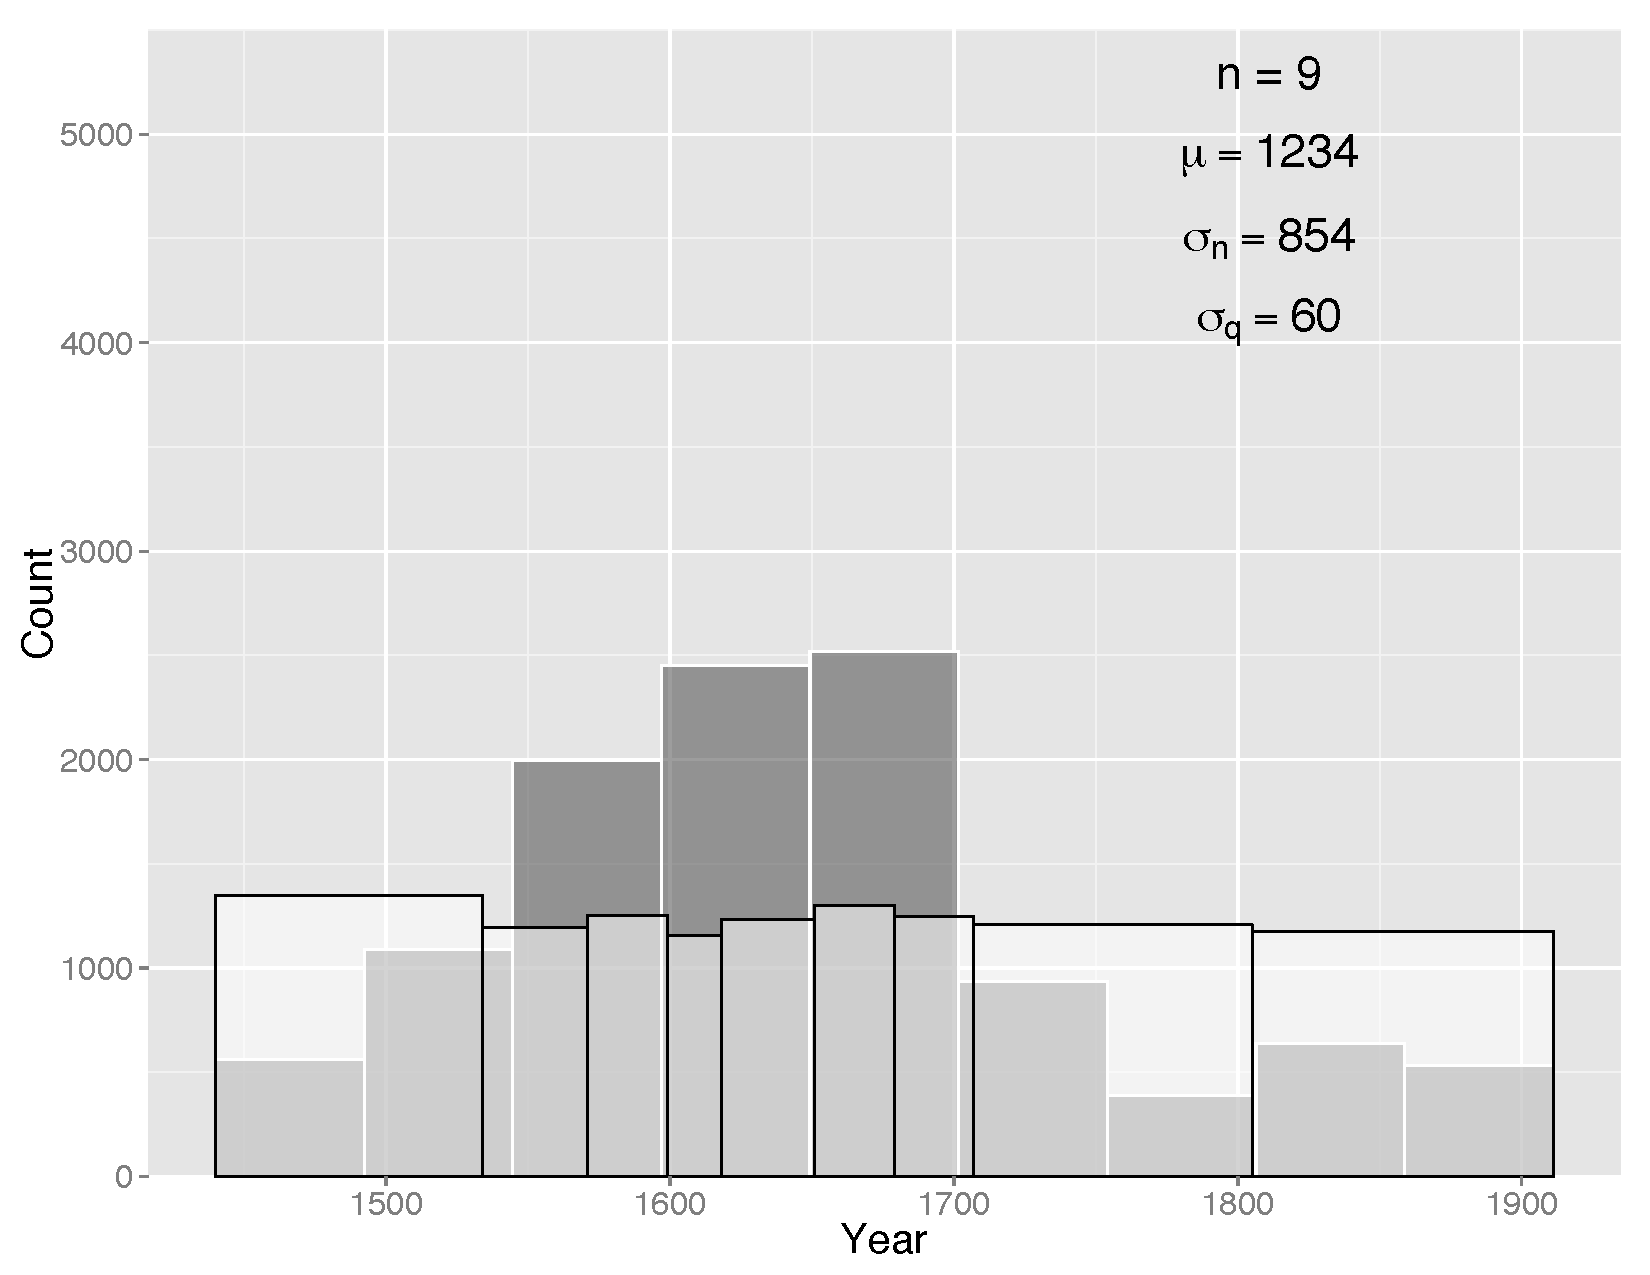
\includegraphics[width=\textwidth]{min-bin-plot.pdf}
%\caption{Finest partition with at least $1000$ tokens per bin.}
%\label{min-bin-plot}
%\end{figure}
%
%
%\section{Correlation}
%
%For variable-width bins, our choice of the exact number of bins is not particularly important. However, we might wonder how we can at least partially motivate not binning too finely. For example, we might consider the number of unique documents per bin for the two methods, as shown in Tables \ref{n-doc} and \ref{q-doc}, or the number of unique authors per bin for the two methods as shown in Tables \ref{n-auth} and \ref{q-auth}. For each number of bins, the table shows the minimum number of documents in a bin, the maximum number of documents in a bin, the mean number of documents in a bin, and the standard deviation of documents per bin.  We could motivate a particular binning using a threshold for the minimum number of documents per bin.
%
%
%
%\begin{table}[ht]
%\centering
%\begin{tabular}{rrrrr}
%  \hline
%Bins & Min & Max & $\mu_d$ & $\sigma_d$ \\ 
%  \hline
%4 & 47 & 1575 & 624.25 & 662.746 \\ 
%  5 & 39 & 1225 & 499.40 & 512.273 \\ 
%  6 & 34 & 1307 & 416.50 & 468.180 \\ 
%  7 & 26 & 1013 & 356.71 & 389.723 \\ 
%  8 & 23 & 1075 & 312.38 & 353.087 \\ 
%  9 & 21 & 879 & 277.78 & 326.295 \\ 
%  10 & 16 & 901 & 250.20 & 286.963 \\ 
%  11 & 18 & 745 & 227.00 & 269.501 \\ 
%  12 & 14 & 789 & 208.67 & 245.017 \\ 
%  13 & 14 & 708 & 192.46 & 239.002 \\ 
%  14 & 10 & 694 & 178.79 & 213.518 \\ 
%  15 & 11 & 641 & 167.00 & 197.391 \\ 
%  16 & 11 & 549 & 156.62 & 186.722 \\ 
%  17 & 9 & 567 & 147.35 & 168.802 \\ 
%  18 & 9 & 552 & 139.22 & 168.018 \\ 
%  19 & 7 & 518 & 131.84 & 156.306 \\ 
%  20 & 5 & 500 & 125.40 & 152.472 \\ 
%   \hline
%\end{tabular}
%\caption{Minimum, maximum, and mean number of \textbf{individual documents} per bin, and standard deviation for \textbf{Fixed-width} bins}
%\label{n-doc}
%\end{table}
%
%\begin{table}[ht]
%\centering
%\begin{tabular}{rrrrr}
%  \hline
%Bins & Min & Max & $\mu_d$ & $\sigma_d$ \\ 
%  \hline
%4 & 92 & 806 & 624.25 & 354.847 \\ 
%  5 & 71 & 875 & 499.20 & 303.735 \\ 
%  6 & 60 & 757 & 416.17 & 292.205 \\ 
%  7 & 43 & 729 & 356.43 & 255.239 \\ 
%  8 & 43 & 568 & 312.62 & 201.626 \\ 
%  9 & 41 & 589 & 278.00 & 211.715 \\ 
%  10 & 32 & 500 & 250.10 & 182.033 \\ 
%  11 & 26 & 484 & 227.36 & 166.642 \\ 
%  12 & 23 & 463 & 208.75 & 161.482 \\ 
%  13 & 13 & 448 & 192.62 & 151.597 \\ 
%  14 & 18 & 426 & 179.00 & 141.207 \\ 
%  15 & 18 & 407 & 167.00 & 132.294 \\ 
%  16 & 11 & 392 & 156.62 & 125.162 \\ 
%  17 & 13 & 392 & 147.35 & 114.299 \\ 
%  18 & 13 & 375 & 139.33 & 115.935 \\ 
%  19 & 2 & 362 & 131.84 & 107.183 \\ 
%  20 & 11 & 344 & 125.45 & 98.628 \\    \hline
%\end{tabular}
%\caption{Minimum, maximum, and mean number of \textbf{individual documents} per bin, and standard deviation for \textbf{Variable-width} bins}
%\label{q-doc}
%\end{table}
%
%\begin{table}[ht]
%\centering
%\begin{tabular}{rrrrr}
%  \hline
%Bins & Min & Max & $\mu_d$ & $\sigma_d$ \\ 
%  \hline
%4 & 43 & 327 & 158.25 & 121.148 \\ 
%  5 & 35 & 235 & 126.20 & 93.138 \\ 
%  6 & 30 & 254 & 107.17 & 83.248 \\ 
%  7 & 23 & 203 & 92.57 & 72.394 \\ 
%  8 & 22 & 202 & 81.62 & 63.859 \\ 
%  9 & 20 & 188 & 74.22 & 61.249 \\ 
%  10 & 15 & 170 & 66.60 & 52.243 \\ 
%  11 & 15 & 159 & 60.45 & 49.800 \\ 
%  12 & 14 & 156 & 57.17 & 47.196 \\ 
%  13 & 14 & 140 & 51.77 & 44.053 \\ 
%  14 & 10 & 142 & 48.86 & 42.551 \\ 
%  15 & 9 & 132 & 45.67 & 38.164 \\ 
%  16 & 8 & 119 & 43.75 & 37.987 \\ 
%  17 & 6 & 120 & 40.76 & 34.052 \\ 
%  18 & 6 & 112 & 39.11 & 33.159 \\ 
%  19 & 6 & 115 & 37.58 & 32.415 \\ 
%  20 & 5 & 109 & 35.80 & 30.753 \\    \hline
%\end{tabular}
%\caption{Minimum, maximum, and mean number of \textbf{individual authors} per bin, and standard deviation for \textbf{Fixed-width} bins}
%\label{n-auth}
%\end{table}
%
%\begin{table}[ht]
%\centering
%\begin{tabular}{rrrrr}
%  \hline
%Bins & Min & Max & $\mu_d$ & $\sigma_d$ \\ 
%  \hline
%4 & 80 & 237 & 162.25 & 64.371 \\ 
%  5 & 63 & 189 & 128.20 & 51.007 \\ 
%  6 & 54 & 183 & 110.33 & 50.674 \\ 
%  7 & 36 & 170 & 95.00 & 47.756 \\ 
%  8 & 37 & 158 & 86.12 & 40.315 \\ 
%  9 & 35 & 149 & 76.22 & 40.969 \\ 
%  10 & 28 & 149 & 68.90 & 37.943 \\ 
%  11 & 24 & 145 & 63.45 & 35.641 \\ 
%  12 & 22 & 143 & 59.58 & 34.857 \\ 
%  13 & 13 & 132 & 54.92 & 32.925 \\ 
%  14 & 17 & 125 & 51.86 & 30.571 \\ 
%  15 & 16 & 123 & 48.13 & 29.640 \\ 
%  16 & 11 & 113 & 46.81 & 27.484 \\ 
%  17 & 13 & 113 & 43.88 & 26.303 \\ 
%  18 & 12 & 106 & 41.94 & 24.981 \\ 
%  19 & 2 & 101 & 39.37 & 24.464 \\ 
%  20 & 10 & 95 & 37.85 & 22.871 \\ 
%   \hline
%\end{tabular}
%\caption{Minimum, maximum, and mean number of \textbf{individual authors} per bin, and standard deviation for \textbf{Variable-width} bins}
%\label{q-auth}
%\end{table}
%
%Making sure that we have a good mix of documents or authors might also allow us to address the problem of autocorrelation. A conservative way of dealing with the potential influence of authorship would be to sample one token per document, and throw out the rest. Using variable-width bins for the sampled tokens ($\sim$ 2500 documents), we obtain the results in Table \ref{sample-q}.\footnote{These data were obtained by setting a random seed and sampling from each document. An absorption event occurs when we have twenty variable-width bins; there is a bin without any instances of \emph{do}-support. Generally speaking, similar results hold for fixed-width bins.}  As a comparison, we can plot the ratio of the p-value of the sampled data to the p-value of the full data as a function of the number of bins as in Figure \ref{doc-sample-q-ratio}. Overlaid on the figure is a box plot of the ratios. Interestingly, sampling a single token from each document does not appear to dramatically alter the results. Since the 
%ratios are not normally distributed, we use the Wilcoxon Signed Rank Test to evaluate whether the mean of the ratios is greater than one. We cannot reject the null hypothesis that the ratios are not greater than one (V = 87, p-value = 0.1742).
%
%\begin{figure}
%\centering
%     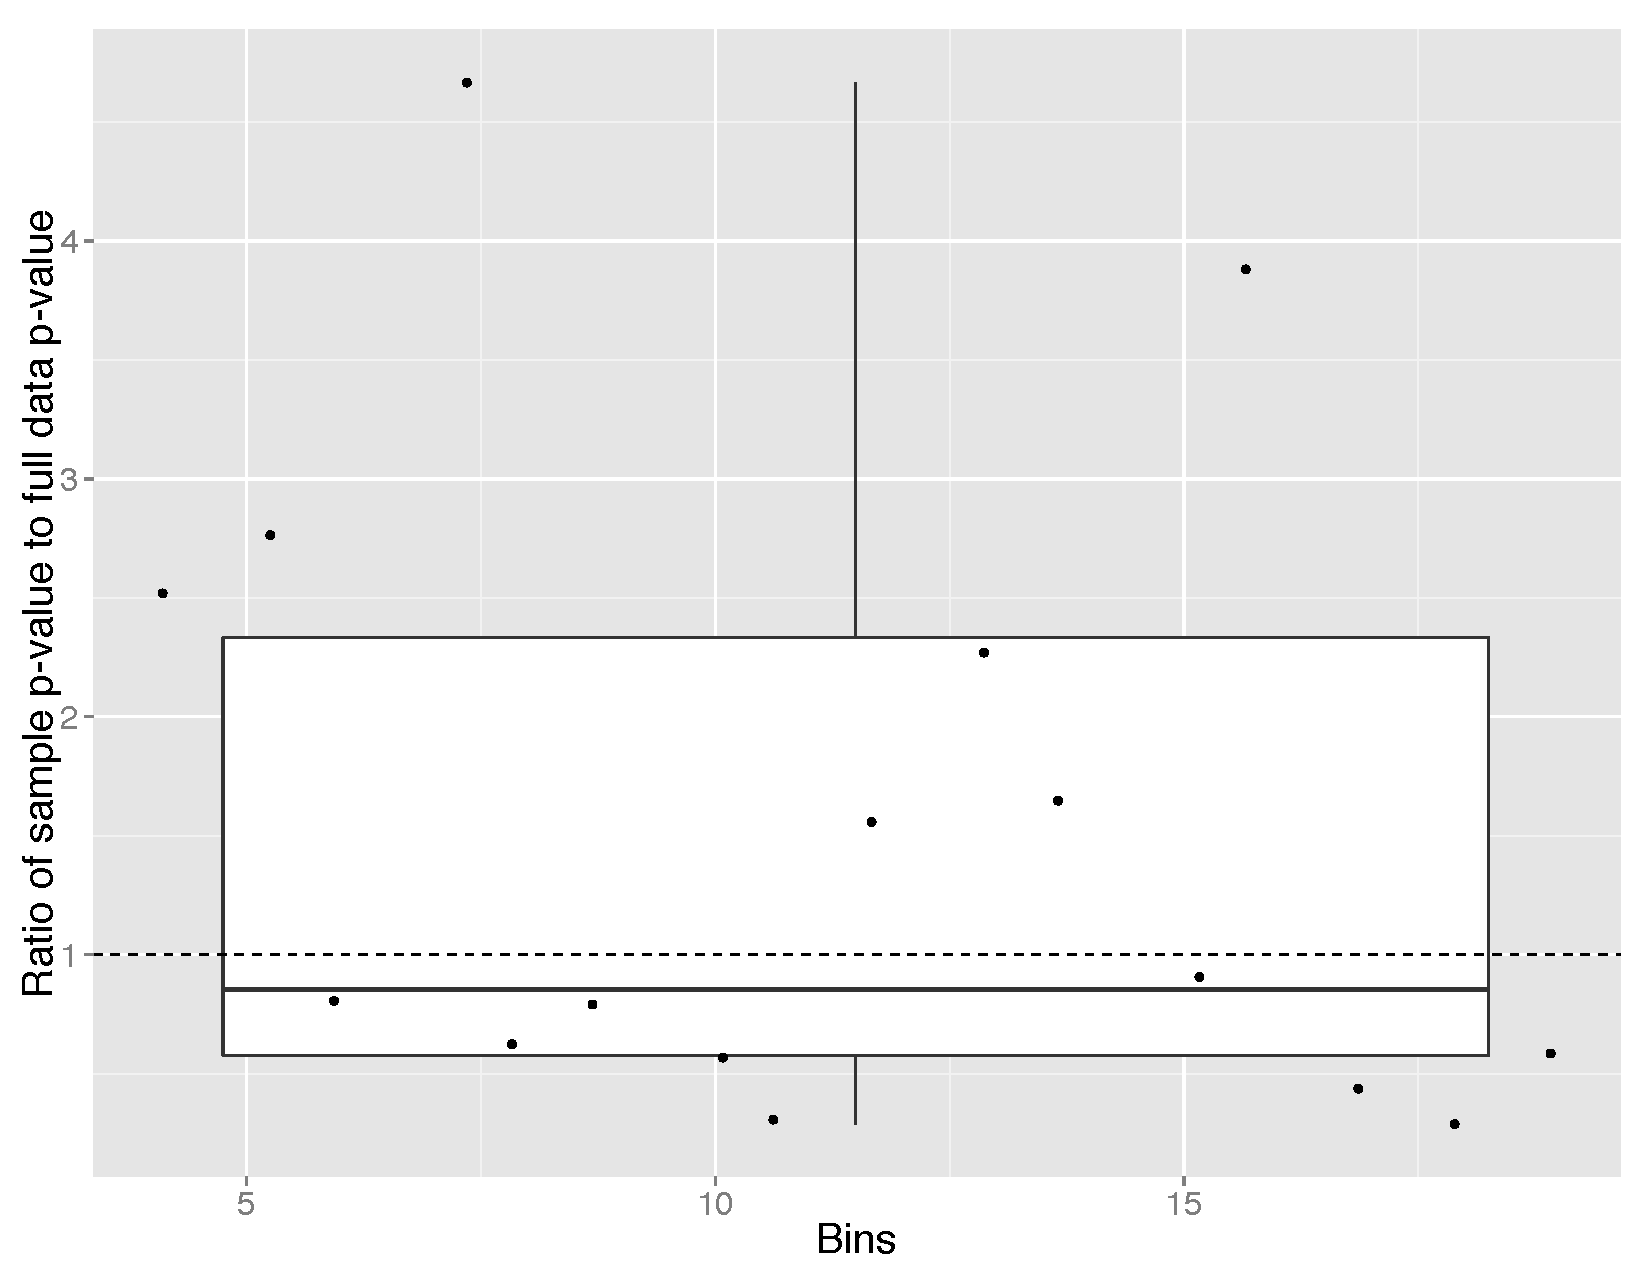
\includegraphics[width=\textwidth]{doc-sample-q-ratio.pdf}
%\caption{Ratio of sample P-value to full data P-value. Dashed line indicates a one to one ratio. The ratios are not significantly greater than one, according to the Wilcoxon Signed Rank Test (V = 87, p-value = 0.1742).}
%\label{doc-sample-q-ratio}
%\end{figure}
%
%
%\begin{table}[ht]
%\centering
%\begin{tabular}{rrrrrrrrrr}
%  \hline
%Bins & ML$s$ & ML$\alpha$ & LRT-P & $\overline{Y}$ & $t_{FI}$ & FIT-P & $\mu$ & $\sigma_q$ & SW-P \\ 
%  \hline
%4 & 0 & 0 & 0 & 0.03588 & 2.40324 & 0.06908 & 623 & 10 & 0.92925 \\ 
%  5 & 0 & 0 & 0 & 0.03548 & 2.67960 & 0.03754 & 498 & 6 & 0.73615 \\ 
%  6 & 0 & 0 & 0 & 0.03619 & 2.33536 & 0.03989 & 415 & 6 & 0.33254 \\ 
%  7 & 0 & 0 & 0 & 0.03699 & 1.97456 & 0.05265 & 356 & 9 & 0.87749 \\ 
%  8 & 0 & 0 & 0 & 0.03105 & 2.52343 & 0.02254 & 311 & 9 & 0.32419 \\ 
%  9 & 0 & 0 & 0 & 0.02782 & 2.62111 & 0.01718 & 276 & 17 & 0.87384 \\ 
%  10 & 0 & 0 & 0 & 0.02468 & 2.84547 & 0.01081 & 249 & 9 & 0.55664 \\ 
%  11 & 0 & 0 & 0 & 0.02464 & 2.70687 & 0.01206 & 226 & 15 & 0.57451 \\ 
%  12 & 0 & 0 & 0 & 0.02336 & 1.86573 & 0.04582 & 207 & 8 & 0.55124 \\ 
%  13 & 0 & 0 & 0 & 0.02544 & 2.11488 & 0.02904 & 191 & 19 & 0.53485 \\ 
%  14 & 0 & 0 & 0 & 0.02641 & 1.73706 & 0.05398 & 178 & 20 & 0.65513 \\ 
%  15 & 0 & 0 & 0 & 0.02273 & 1.92467 & 0.03822 & 166 & 10 & 0.83400 \\ 
%  16 & 0 & 0 & 0 & 0.02069 & 1.60461 & 0.06545 & 155 & 11 & 0.88421 \\ 
%  17 & 0 & 0 & 0 & 0.01868 & 2.34282 & 0.01667 & 146 & 18 & 0.34093 \\ 
%  18 & 0 & 0 & 0 & 0.01917 & 2.42347 & 0.01380 & 138 & 16 & 0.64276 \\ 
%  19 & 0 & 0 & 0 & 0.02025 & 1.84180 & 0.04151 & 131 & 15 & 0.57947 \\ 
%   \hline
%\end{tabular}
%\label{sample-q}
% \caption{Variable-width bins for \textbf{All \emph{do}-support data} with one token sampled from each \textbf{document}.}
%\end{table}
%
%In fact, we can be even more conservative, and sample only a single token from each author as is shown in Table \ref{auth-sample-q-ratio}.\footnote{Here, we can only proceed up to twelve bins due to an absorption event in the second to last bin. Similar results hold for fixed-width bins. This actually underestimates the number of authors, possibly by around fifty.} We cannot bin as finely given that we have fewer authors ($\sim$ 600 authors). However, again, the same general result holds.
%Again, since the ratios are not normally distributed, we use the Wilcoxon Signed Rank Test to evaluate whether the mean of the ratios is greater than one. We cannot reject the null hypothesis that the ratios are not greater than one  (V = 18, p-value = 0.7148).   Given that throwing out most of the data does not affect the results, we can be reasonably confident that the effect of individual authorship is not problematic.
%
%\begin{table}[ht]
%\centering
%\begin{tabular}{rrrrrrrrrr}
%  \hline
%Bins & ML$s$ & ML$\alpha$ & LRT-P & $\overline{Y}$ & $t_{FI}$ & FIT-P & $\mu$ & $\sigma_q$ & SW-P \\ 
%  \hline
%4 & 0 & 0 & 0 & 0.04278 & 2.37747 & 0.07028 & 151 & 2 & 0.83772 \\ 
%  5 & 0 & 0 & 0 & 0.03982 & 2.71884 & 0.03631 & 120 & 3 & 0.39502 \\ 
%  6 & 0 & 0 & 0 & 0.03700 & 3.25883 & 0.01556 & 100 & 1 & 0.86116 \\ 
%  7 & 0 & 0 & 0 & 0.03287 & 2.97072 & 0.01557 & 86 & 2 & 0.90967 \\ 
%  8 & 0 & 0 & 0 & 0.02972 & 2.88301 & 0.01397 & 75 & 2 & 0.48000 \\ 
%  9 & 0 & 0 & 0 & 0.02745 & 3.17303 & 0.00782 & 67 & 3 & 0.59353 \\ 
%  10 & 0 & 0 & 0 & 0.02659 & 3.14573 & 0.00684 & 60 & 3 & 0.73464 \\ 
%  11 & 0 & 0 & 0 & 0.02682 & 2.72904 & 0.01163 & 54 & 2 & 0.59698 \\ 
%  12 & 0 & 0 & 0 & 0.02481 & 3.22867 & 0.00452 & 50 & 1 & 0.96526 \\ 
%   \hline
%\end{tabular}
% \caption{Variable-width bins for \textbf{All \emph{do}-support data} with one token sampled from each \textbf{author}.}
%\end{table}
%
%\begin{figure}
%\centering
%     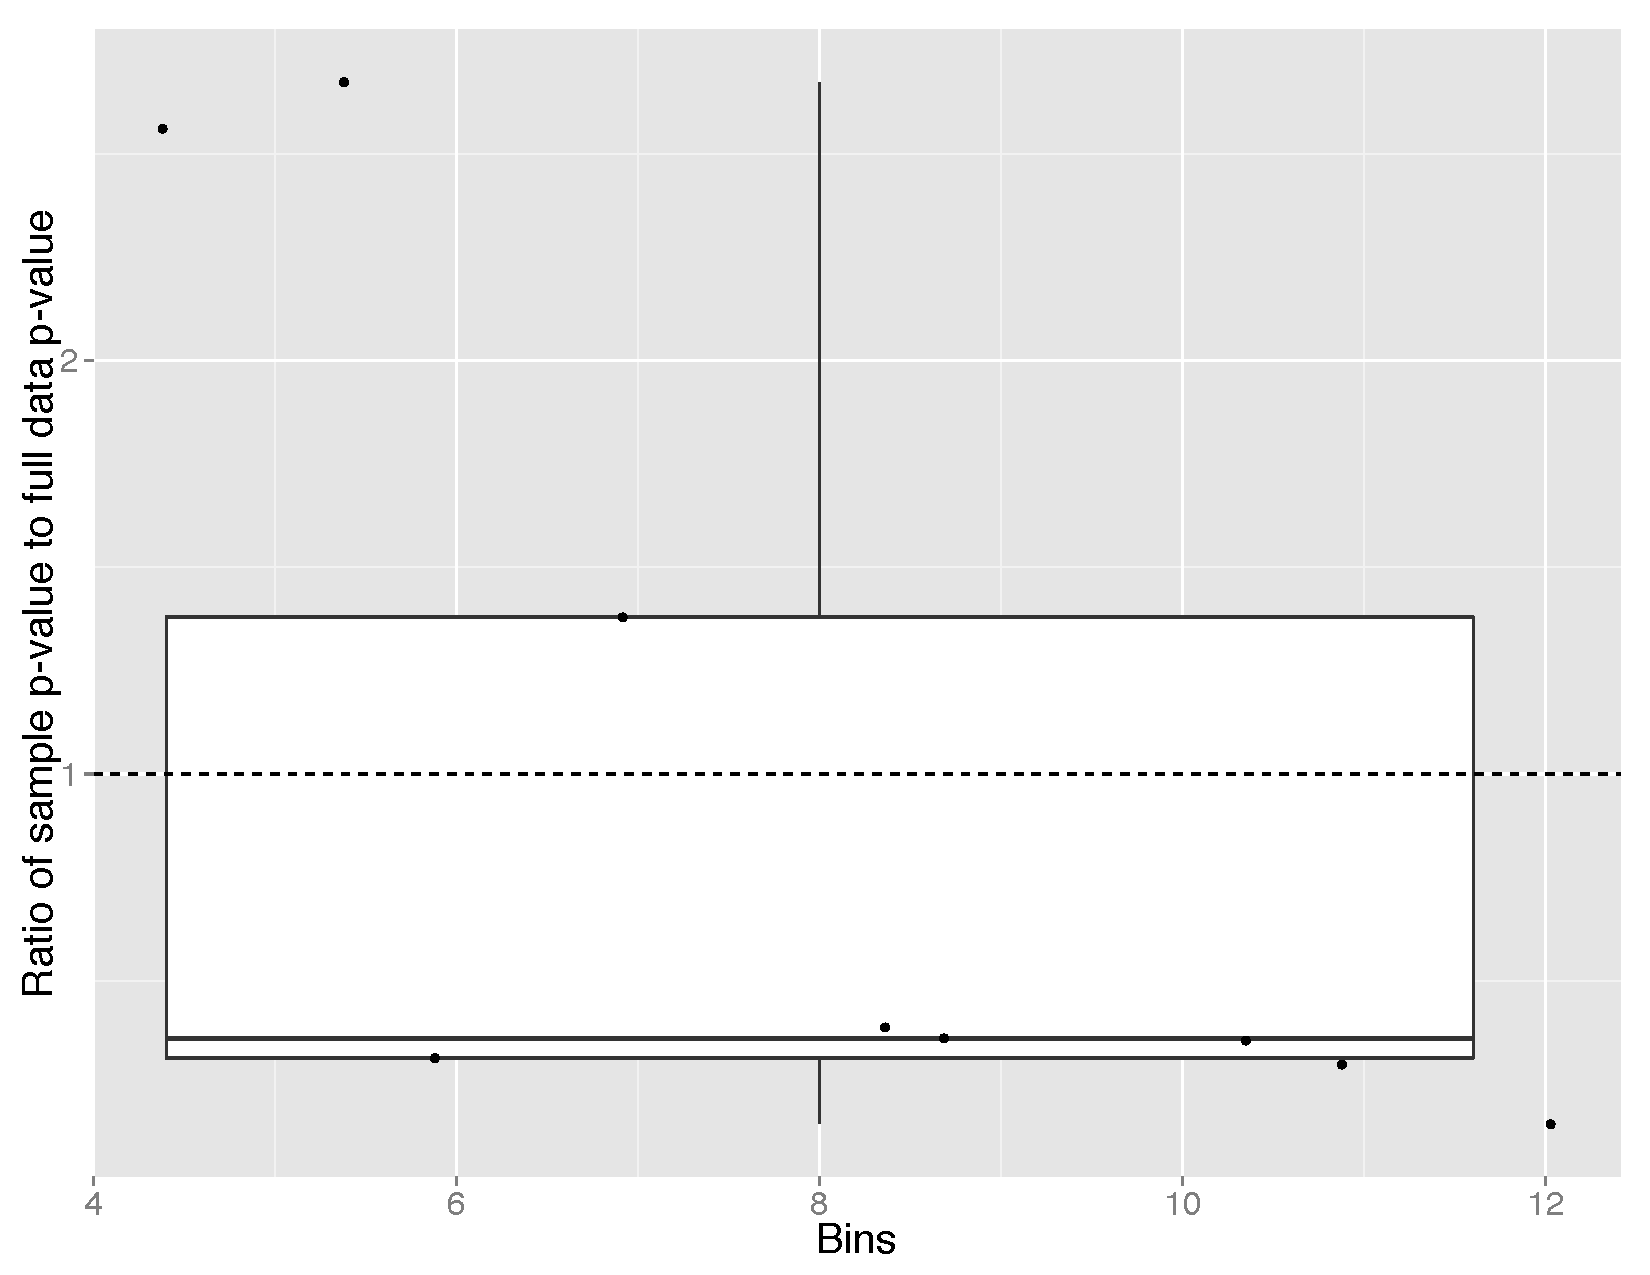
\includegraphics[width=\textwidth]{auth-sample-q-ratio.pdf}
%\caption{Ratio of sample P-value to full data P-value. Dashed line indicates a one to one ratio. The ratios are not significantly greater than one, according to the Wilcoxon Signed Rank Test (V = 18, p-value = 0.7148).}
%\label{auth-sample-q-ratio}
%\end{figure}